\chapter{Temperatures and timescales of methane synthesis and hydrogen exchange at oceanic spreading centers} \label{ch:3}
%\chaptermark{Methane synthesis and hydrogen exchange at oceanic spreading centers}
\chaptermark{Mid-ocean ridge hydrothermal systems}

\begin{abstract}
\noindent Hot-spring fluids emanating from deep-sea hydrothermal systems hosted in
unsedimented mafic and ultramafic rock commonly contain high
concentrations of methane. Multiple hypotheses have been proposed for
the origin(s) of this methane, ranging from synthesis via reduction of
aqueous inorganic carbon ($\big\sum\!$CO\textsubscript{2}) during active fluid circulation to leaching of
methane-rich fluid inclusions formed in plutonic rocks at depth. To
further resolve the mechanism(s) responsible for methane generation in
these systems, we determined the relative abundances of several methane
isotopologues (including \textsuperscript{13}CH\textsubscript{3}D, a
``clumped'' isotopologue containing two rare isotope substitutions) in
geochemically diverse fluids sampled at the Rainbow, Von Damm, Lost
City, and Lucky Strike hydrothermal vent fields.

The methane clumped isotopologue data indicate relatively uniform
apparent equilibrium temperatures (averaging \(310_{- 42}^{+ 53}\)~°C)
across the suite of endmember fluids, with no apparent relation to the wide range
of fluid temperatures (96 to 370~°C), chemical compositions (pH,
{[}H\textsubscript{2}{]}, {[}$\big\sum\!$CO\textsubscript{2}{]},
{[}CH\textsubscript{4}{]}), and geologic settings represented. Combined
with similar stable isotope ratio
(\textsuperscript{13}C/\textsuperscript{12}C and D/H) of methane, all
available geochemical and isotopic data suggest a common mechanism of
methane generation at depth, independent of actively-circulating
hydrothermal fluids. Apparent isotopologue equilibrium at temperatures
of ca.\ 270 to 360~°C indicates that hydrogen-isotope exchange
is sluggish for methane at temperatures below 270~°C here.  The isotopologue data are
compatible with the thermodynamically-favorable reduction of
CO\textsubscript{2}(\emph{g}) to CH\textsubscript{4}(\emph{g}) at
temperatures below ca.\ 500~°C under redox conditions characterizing
intrusive rocks derived from subridge melts. These results provide
further evidence that low temperature (\textless{}200~°C) water rock
reaction does not contribute significantly to the quantities of methane
venting at the seafloor in mid-ocean ridge hot springs, and suggest that
 methane forms from respeciation of
magmatic volatiles occluded in plutonic rocks of the oceanic crust, and
are later leached during convective hydrothermal circulation.
\end{abstract}

\vspace*{\fill}

\noindent \rule{\textwidth}{0.4pt}\\

{\small
	
	\noindent A version of this chapter is being prepared as a manuscript by the following authors:\\
	
	\noindent David T. Wang\textsuperscript{a,b,}*, Eoghan P.
	Reeves\textsuperscript{a,b,c}, Jeffrey S. Seewald\textsuperscript{b},
	Jill M. McDermott\textsuperscript{a,b,d}, and Shuhei
	Ono\textsuperscript{a}\\
	
	\begin{itemize}[labelsep*=1pt, leftmargin=10pt]
		\item[\tss a] Department of Earth, Atmospheric and Planetary Sciences, Massachusetts Institute of Technology, Cambridge, Massachusetts 02139, USA.
		\item[\tss b] Marine Chemistry and Geochemistry Department, Woods Hole Oceanographic Institution, Woods Hole, Massa\-chu\-setts 02543, USA.
		\item[\tss c] Department of Earth Science and Centre for Geobiology, University of Bergen, Bergen N-5020, Norway.
		\item[\tss d] Earth and Environmental Sciences Department, Lehigh University, Bethlehem, Pennsylvania 18015, USA.
		\item[*] To whom correspondence should be addressed. {\itshape E-mail}: \href{mailto:dtw@alum.mit.edu}{\nolinkurl{dtw@alum.mit.edu}} (D.T.W.)
	\end{itemize}

}

\clearpage

\section{Introduction} \label{sec:3:intro}

Dissolved methane (CH\textsubscript{4}) is ubiquitous in hot spring
fluids emanating from submarine hydrothermal vents, and is a potential
carbon source for microbial communities living at and below the seafloor
and in the water column. Constraining the sources of carbon (C) and
hydrogen (H) for the production of CH\textsubscript{4}, as well as the
depths and temperatures at which CH\textsubscript{4} is generated in
these hydrothermal systems, is critical for understanding the origin of
methane \parencite{Welhan_1988_CG,Charlou++_2002_CG,Proskurowski++_2008_S,McDermott++_2015_PNAS}. The abundance and isotopic composition of
methane venting from submarine hydrothermal fields that are relatively
free of sediment cover has been described at oceanic spreading centers
characterized by a range of spreading rates \parencite[e.g.,][]{Welhan_1988_CG,Charlou++_2002_CG,McCollom+Seewald_2007_CR,Proskurowski++_2008_S,Cannat++_2010,Charlou++_2010,Proskurowski_2010,McDermott++_2015_PNAS,McDermott_2015_thesis}. In general, fluids that
have interacted with ultramafic rocks are substantially enriched in
CH\textsubscript{4} relative to fluids that have reacted with mafic
rocks \parencite{Keir_2010_GRL}, although there are exceptions in which high-CH\textsubscript{4} fluids are associated with apparent mafic substrates (e.g., basalt)
\parencite{Charlou++_2000_CG}.

Several distinct geochemical processes have been proposed to account for
the presence of abiotic CH\textsubscript{4} in submarine hydrothermal
fluids. Some have proposed that CH\textsubscript{4} is formed by
reduction of aqueous inorganic carbon (i.e., $\big\sum\!$CO\textsubscript{2}) in
subsurface reaction zones during convective circulation of
seawater-derived hydrothermal vent fluids in response to the highly
reducing (H\textsubscript{2}-rich) conditions that result from extensive
fluid-mineral interactions during serpentinization of ultramafic rock
\parencite{Charlou++_2002_CG,Proskurowski++_2008_S}. Experimental studies
showed, however, that aqueous reduction of $\big\sum\!$CO\textsubscript{2} to
CH\textsubscript{4} is slow under conditions thought to occur naturally
in ultramafic hydrothermal systems \parencite{McCollom+Seewald_2001_GCA,McCollom_2016_PNAS}.

Earlier studies have shown that plutonic (gabbroic) rocks from the ocean floor
contain copious amounts of methane \parencite{Kelley_1996_JGR,Kelley_1997,Kelley+FruhGreen_1999_JGR}. These authors suggested a model
involving entrapment and respeciation of fluids that contained
mantle-derived CO\textsubscript{2} into fluids rich in CH\textsubscript{4}
(±~graphite) within gabbros, and subsequent extraction of the
CH\textsubscript{4} during hydrothermal circulation \parencite{McDermott++_2015_PNAS}. Leaching of basalt-hosted gas vesicles that contain
CH\textsubscript{4} may also be a source of CH\textsubscript{4} in
fluids venting at fast-spreading ridges such as the East Pacific Rise \parencite{Welhan+Craig_1983,Welhan_1988_CJES}.

To constrain the origin of methane in unsedimented submarine
hydrothermal systems, we determined the relative abundance of four
stable isotopologues of methane
(\textsuperscript{12}CH\textsubscript{4},
\textsuperscript{13}CH\textsubscript{4},
\textsuperscript{12}CH\textsubscript{3}D, and
\textsuperscript{13}CH\textsubscript{3}D, a doubly-substituted or
``clumped'' isotopologue) in a diverse set of fluids collected from four
hydrothermal vent fields: Rainbow (\ang[minimum-integer-digits=2]{36;13;48}N, \ang[minimum-integer-digits=2]{33;54;09}W,
Mid-Atlantic Ridge), Von Damm (\ang[minimum-integer-digits=2]{18;22;36}N, \ang{81;47;54}W, Mid-Cayman
Rise), Lost City (\ang[minimum-integer-digits=2]{30;07;24}N, \ang[minimum-integer-digits=2]{42;07;12}W, Mid-Atlantic Ridge), and
Lucky Strike (\ang[minimum-integer-digits=2]{37;17;30}N, \ang[minimum-integer-digits=2]{32;16;42}W, Mid-Atlantic Ridge). Fluids
from these fields span a wide range of temperatures (96 to 370~°C) and
represent distinct geochemical regimes and geological settings.

Data presented in this study provide constraints on the sources of C and
H in methane, as well as temperature(s) associated with the formation or
equilibration of the C--H bonds. Carbon- and hydrogen-isotope ratios
encode signals related to the sources of C and H, respectively, as well
as isotopic fractionations incurred during the synthesis of methane.
Complementary to such information, measurement of methane clumped
isotopologues provides an independent estimate of the temperature at
which the C--H bonds in methane were formed or last equilibrated \parencite{Stolper++_2014_S,Wang++_2015_S}. Constraining the temperatures
at which methane synthesis occurs within oceanic crust has direct
implications for the distribution and availability of reduced carbon
substrates and energy sources that may support a deep biosphere, as well
as for the transfer of mantle-derived carbon to the Earth's surface.

Determination of temperatures from carbon or hydrogen isotope ratios of
methane alone requires knowledge of or assumptions regarding the
isotopic composition of other species with which methane has exchanged C
or H (e.g., CO\textsubscript{2} or H\textsubscript{2}O). In contrast,
temperatures determined from the abundance of
\textsuperscript{13}CH\textsubscript{3}D do not require information
regarding such coexisting species. Thus, clumped isotopologue data in
conjunction with carbon- and hydrogen-isotope ratios of methane can be
used to constrain the isotopic compositions of C- and H-bearing species
associated with the methane source when independent constraints are
unavailable. In the following discussion, we show how clumped
isotopologue temperatures of methane, together with bulk
\textsuperscript{13}C/\textsuperscript{12}C and D/H isotope ratios,
fluid chemistry, and thermodynamic considerations, collectively indicate
that methane in unsedimented hydrothermal systems originates at high
temperatures of (ca.\ 250 to 400~°C) and constrain possible environments
of methane generation.

\section{Methods}\label{methods}

\subsection{Vent fluid samples}\label{vent-fluid-samples}

The fluid samples studied herein were collected by ROV \emph{Jason II}
using isobaric gas-tight samplers \parencite{Seewald++_2002_DSR} during cruises
to the Mid-Atlantic Ridge in 2008 and Mid-Cayman Rise in 2012. During
subsampling of the vent fluids from the samplers, fluid samples were
stored in pre-evacuated serum vials and sealed with blue butyl rubber
stoppers that were boiled in 2 M NaOH for 2--4 hours and rinsed in
deionized water prior to use. When necessary, sample aliquots in
multiple serum vials were combined (``pooled'') prior to purification to
obtain enough CH\textsubscript{4} for clumped isotopologue analysis.
When possible, aliquots from the same fluid sampler were used. In some
cases, however, it was necessary to combine aliquots from duplicate
samples collected in separate samplers deployed in the same hydrothermal
fluid during a submersible dive (\autoref{tab:3:1}). Due to the exceedingly low
concentration of dissolved CH\textsubscript{4} in ambient bottom
seawater \parencite[\textless{}10\textsuperscript{$-$8}~M,][]{McDermott++_2015_PNAS,Reeves++_2014_PNAS} relative to concentrations in endmember vent fluids
(samples regressed to zero Mg content) (\autoref{tab:3:2}), inadvertent
entrainment of seawater during fluid collection has no effect on the
isotopic composition of vent-fluid derived methane measured during this
study.

\subsection{Analytical techniques}\label{analytical-techniques}

Samples of methane were purified via cryofocusing--preparative gas
chromatography \parencite{Wang++_2015_S}. The relative abundances of the
methane stable isotopologues \textsuperscript{12}CH\textsubscript{4},
\textsuperscript{13}CH\textsubscript{4},
\textsuperscript{12}CH\textsubscript{3}D, and
\textsuperscript{13}CH\textsubscript{3}D were measured using a tunable
infrared laser direct absorption spectroscopy technique described
previously \parencite{Ono++_2014_AC,Wang++_2015_S}. Due to the small
amounts of CH\textsubscript{4} (ca.\ 1~cm\textsuperscript{3} STP) in
samples analyzed as part of this study, a cold trap system was employed
to recover and recycle gas samples for re-analysis \parencite{Wang++_2015_S}.
A set of samples with previously-determined isotopologue ratios was also
re-measured using the recycling technique, to verify accuracy.

The abundance of \textsuperscript{13}CH\textsubscript{3}D relative to a
random distribution of isotopes among the isotopologues (stochastic
distribution) is tracked using the metric
Δ\textsuperscript{13}CH\textsubscript{3}D, which is defined as:
Δ\textsuperscript{13}CH\textsubscript{3}D = ln \emph{Q} (or nearly
equivalently, \emph{Q} -- 1), where \emph{Q} is the reaction quotient of
the isotope exchange reaction:
\begin{equation}\label{eqn:3:1}
{}^{13}\text{CH}_4+ {}^{12}{\text{CH}}_3\text{D}\rightleftharpoons {}^{13}{\text{CH}}_3\text{D}+ {}^{12}{\text{CH}}_4
\end{equation}

Values of Δ\textsuperscript{13}CH\textsubscript{3}D \textgreater{} 0‰
are used to calculate apparent equilibrium temperatures
(\emph{T}\textsubscript{13D}) using the calibration of \textcite{Wang++_2015_S}, which is based on quantum chemical predictions for methane
isotopologues in the gas phase and anchored by measurements of methane
samples heated in the presence of catalyst at temperatures between 150 and 400~°C.

\begin{table}

	\centering
	
	\caption[Isotopic and isotopologue ratios of methane in studied hydrothermal fluids]{Carbon and hydrogen isotope ratios and clumped isotopologue abundances
	of methane in studied hydrothermal fluids.}
	\label{tab:3:1}

	\begin{threeparttable}
	
		\begin{tabular}[]{@{} l l l @{} r r >{\raggedleft\arraybackslash}p{2.5em}@{\hspace{0.2em}}l r@{\hspace{0.2em}}l @{}}
			\toprule
			{Field} & Vent & Sample(s) & δ\textsuperscript{13}C (‰) & δD (‰)
			& \multicolumn{2}{c}{Δ\textsuperscript{13}CH\textsubscript{3}D (‰)} &
			\multicolumn{2}{c}{\emph{T}\textsubscript{13D} (°C)}\tabularnewline
			\midrule
		%	\endhead
			{Rainbow} & Guillaume & J2-352-IGT4 & $-$17.6 & $-$97.7 &
			\textbf{0.95} & ± 0.60 & \textbf{450} & +298/$-$136\tabularnewline
			& CMSP\&P & J2-354-IGT3 & $-$17.5 & $-$97.8 & \textbf{1.50} & ± 0.60 &
			\textbf{322} & +142/$-$85\tabularnewline
			& Auberge & J2-352-IGT3 & $-$17.4 & $-$97.9 & \textbf{1.73} & ± 0.60 &
			\textbf{285} & +114/$-$73\tabularnewline
			{Von Damm} & Old Man Tree\textsuperscript{a} & J2-612-IGT6/-IGT8
			& $-$16.2 & $-$107.4 & \textbf{1.71} & ± 0.35 & \textbf{288} &
			+60/$-$47\tabularnewline
			& Ravelin 1 & J2-617-IGT6 & $-$16.4 & $-$106.6 & \textbf{1.56} & ± 0.60 &
			\textbf{312} & +134/$-$82\tabularnewline
			& East Summit & J2-612-IGT2 & $-$16.4 & $-$106.5 & \textbf{1.35} & ± 0.60 &
			\textbf{350} & +167/$-$95\tabularnewline
			{Lost City} & Beehive & J2-361-IGT5/-CGTWu & $-$10.9 & $-$126.6 &
			\textbf{1.84} & ± 0.60 & \textbf{270} & +104/$-$68\tabularnewline
			{Lucky Strike} & Medea\textsuperscript{a} & J2-359-IGT2/-CGTY &
			$-$14.2 & $-$99.3 & \textbf{1.63} & ± 0.40 & \textbf{301} &
			+75/$-$55\tabularnewline
			& Isabel\textsuperscript{a} & J2-357-IGT5/-CGTY & $-$12.6 & $-$100.4 &
			\textbf{1.85} & ± 0.30 & \textbf{269} & +45/$-$37\tabularnewline
			\bottomrule
		\end{tabular}
		
		\begin{tablenotes}
			\item Values for δ\textsuperscript{13}C, δD, and
			Δ\textsuperscript{13}CH\textsubscript{3}D are reported relative to
			Vienna Pee Dee Belemnite (VPDB), Vienna Standard Mean Ocean Water
			(VSMOW), and the stochastic distribution, respectively. Analytical
			uncertainties for δ\textsuperscript{13}C and δD are both ca.\ ±0.1‰ (95\%
			confidence intervals). Uncertainties listed for
			Δ\textsuperscript{13}CH\textsubscript{3}D and
			\emph{T}\textsubscript{13D} are 95\% confidence intervals; the last
			digit in each (hundredths and ones places, respectively) is not
			significant.
			
			\item \textsuperscript{a} Samples analyzed in duplicate. Uncertainties listed
			are 2 s.e.m.\ (standard error of the mean) of the replicate measurements
			(\emph{n} = 2).
		
		\end{tablenotes}
	
	\end{threeparttable}

\end{table}

Isotope values are reported using standard delta-notation, i.e.,
δ\textsuperscript{13}C =
(\textsuperscript{13}C/\textsuperscript{12}C)\textsubscript{sample}/(\textsuperscript{13}C/\textsuperscript{12}C)\textsubscript{VPDB}
$-$ 1, and δD = (D/H)\textsubscript{sample}/(D/H)\textsubscript{VSMOW} --
1. The permil (‰) symbol represents multiplication by
10\textsuperscript{$-$3}; hence, we have omitted the factor of 1000
commonly seen in definitions of δ and other isotope values. The
δ\textsuperscript{13}C and δD values are calibrated against community
reference gases NGS-1 and NGS-3 \parencite{Wang++_2015_S}.

\section{Results}\label{sec:3:results}

Results of stable carbon (\textsuperscript{13}C/\textsuperscript{12}C)
and hydrogen (D/H) isotope ratio measurements are shown in \autoref{tab:3:1}.
These results are in general agreement with previously-published methane
isotopic data for these samples or systems \parencite{Proskurowski++_2008_S,Charlou++_2010,Pester++_2012_GCA,McDermott++_2015_PNAS}.
Similar values were observed across the different hydrothermal fields,
ranging from $-$18‰ to $-$11‰ in δ\textsuperscript{13}C and $-$127‰ to $-$98‰ in
δD. Variation between vents in the same field (generally \textless{}1‰
in both δ\textsuperscript{13}C and δD) is significantly smaller than
variation across different fields. The consistency of stable isotope
data within each field is added evidence for the interpretations
previously drawn of conservative mixing of CH\textsubscript{4} between
bottom seawater and a single CH\textsubscript{4}-bearing endmember fluid
at Rainbow \parencite{Charlou++_2002_CG} and Von Damm \parencite{McDermott++_2015_PNAS}.
A common source fluid has also been suggested for Lucky Strike \parencite{Pester++_2012_GCA} and Lost City \parencite{Seyfried++_2015_GCA} based on the
compositions of fluids there.


\begin{SCfigure*}
	\centering
	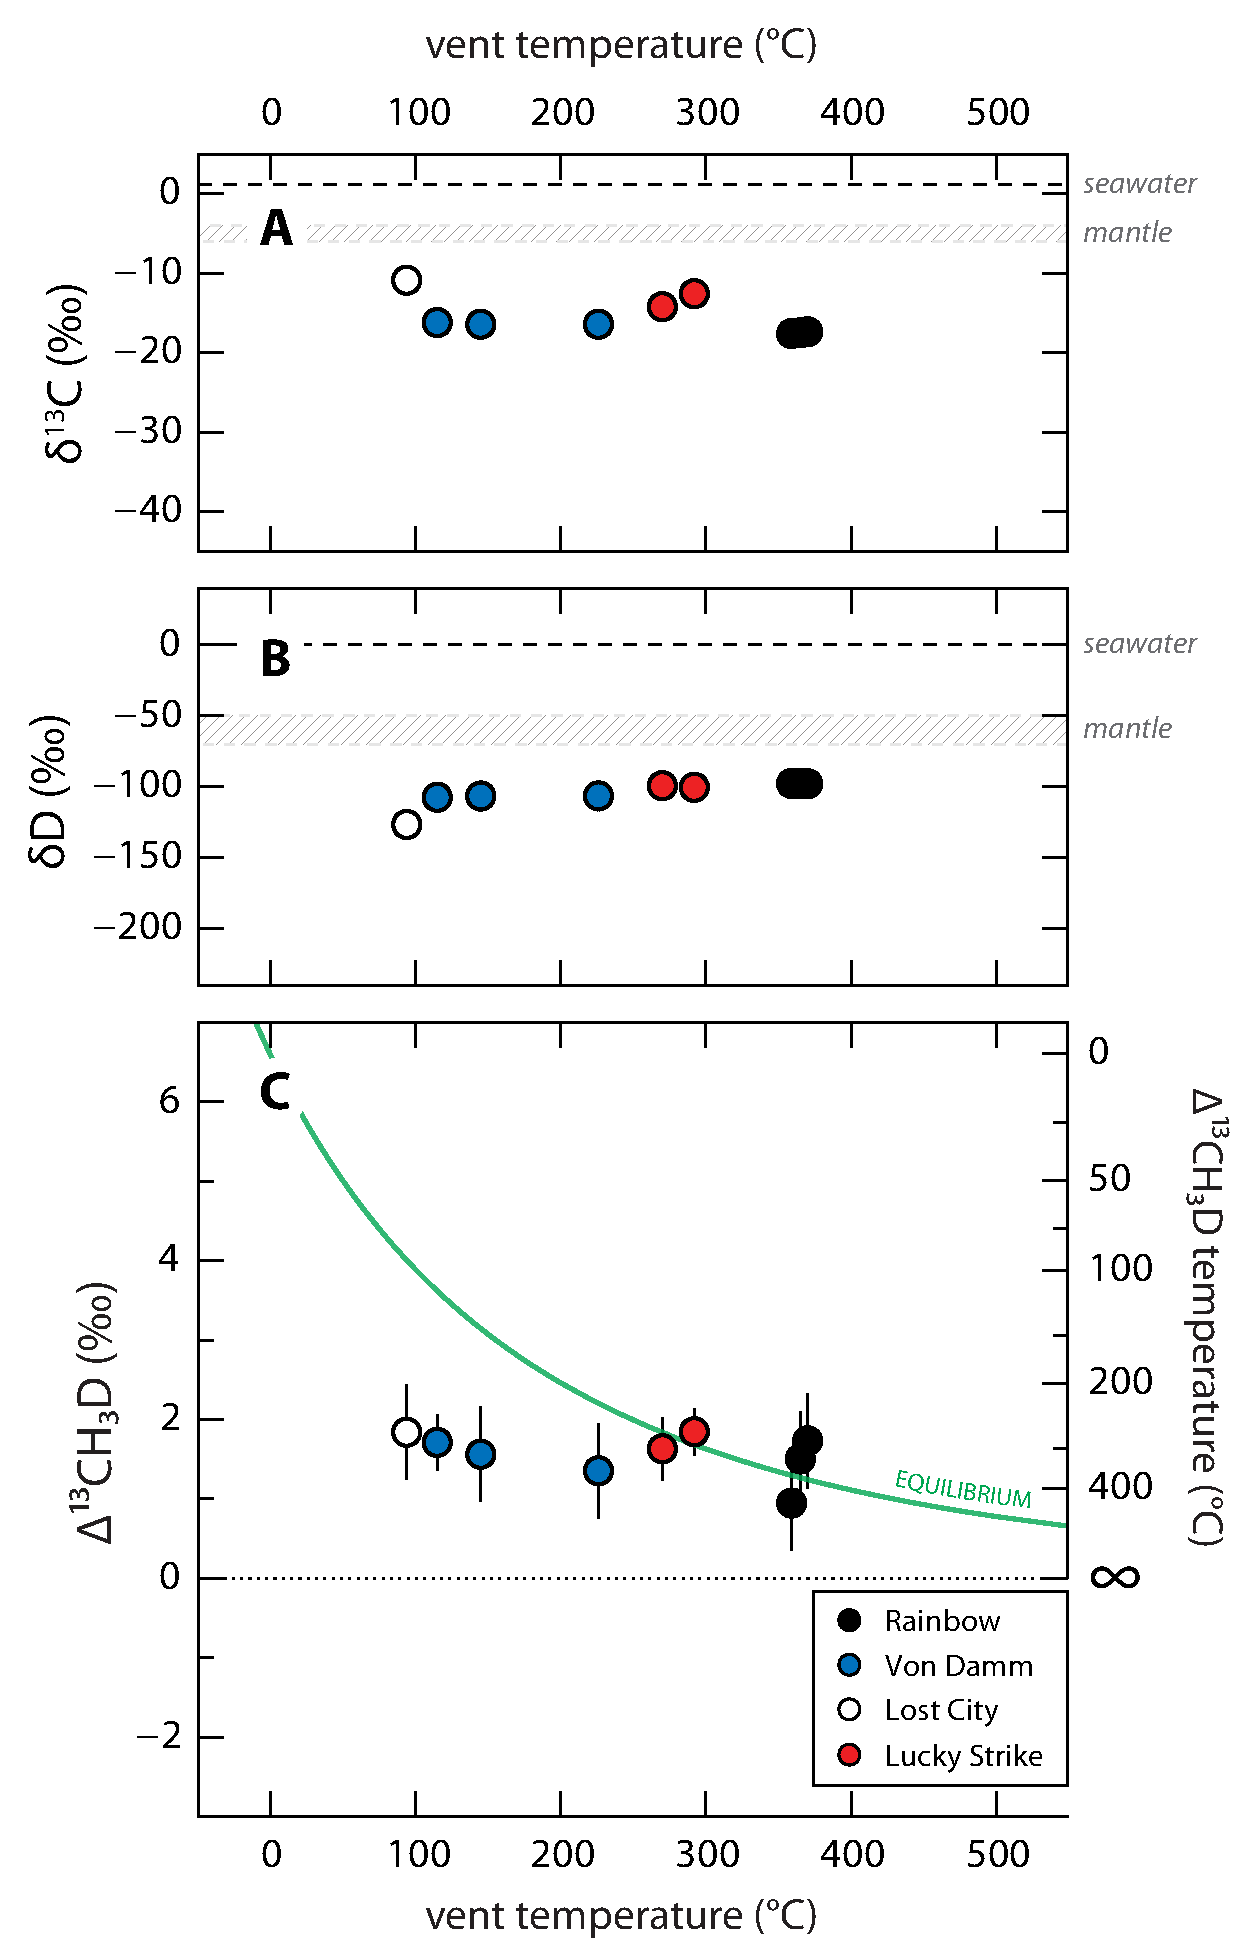
\includegraphics[width=0.6\linewidth]{figures/Fig3.1}
	\caption[Isotope and isotopologue ratios of methane at studied vent sites]{%
		Comparison of (\textbf{A}) δ\textsuperscript{13}C, (\textbf{B}) δD, and
		(\textbf{C}) Δ\textsuperscript{13}CH\textsubscript{3}D values of methane
		across vent sites. Data and error bars (95\% confidence interval) are
		from \autoref{tab:3:1}. In all panels, points are plotted against measured vent
		temperature (\autoref{tab:3:2}). The isotopic compositions of inorganic carbon (A)
		and hydrogen (B) in seawater and in the mantle are shown \parencite{Javoy++_1986_CG,Blank++_1993_GCA,Clog++_2013_EPSL}. In (C), the green line
		represents the clumped isotopologue composition at equilibrium. The
		Δ\textsuperscript{13}CH\textsubscript{3}D temperature scale corresponds
		to the calibration from \textcite{Wang++_2015_S}.
	}
	\label{fig:3:1}
\end{SCfigure*}


\begin{figure*}
	\centering
	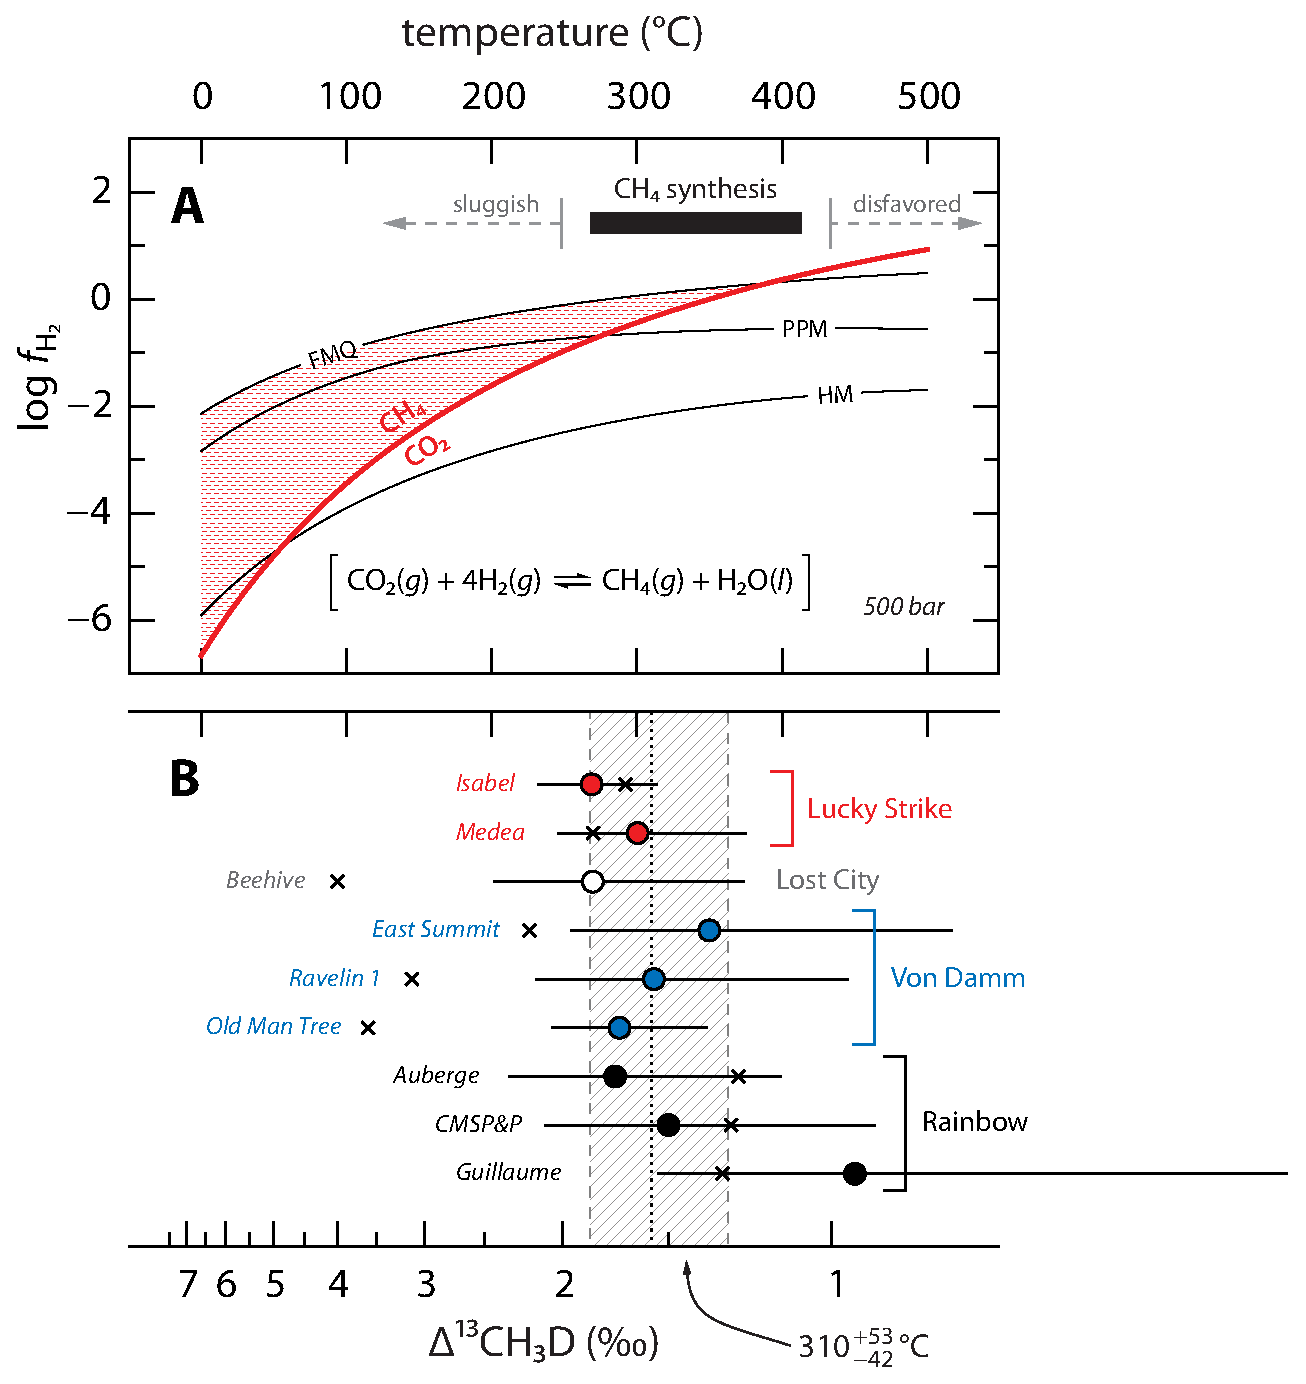
\includegraphics[width=0.75\linewidth]{figures/Fig3.2}
	\caption[Constraints on methane formation and stability from thermodynamics and
	clumped isotopologues]{%
		Constraints on methane formation and stability from thermodynamics and
		clumped isotopologue data. (\textbf{A}) Plot of fugacity of
		H\textsubscript{2} as a function of temperature at 500 bar, after \textcite{Shock_1992}. Red line represents the fugacity of H\textsubscript{2} at
		equilibrium, according to the reaction $ \ce{CO2\text{(\emph{g})}} + 4\ce{H2\text{(\emph{g})}} \leftrightharpoons
\ce{CH4\text{(\emph{g})}} + 2\ce{H2O\text{(\emph{l})}} $, when the fugacities of
		CH\textsubscript{4} and CO\textsubscript{2} are equal, and assuming unit
		activity for H\textsubscript{2}O(\emph{l}). Grey lines represent
		equilibrium H\textsubscript{2} fugacities buffered by the mineral
		assemblages fayalite-magnetite-quartz (FMQ), pyrite-pyrrhotite-magnetite
		(PPM), and hematite-magnetite (HM). Red shaded area represents the
		intersection of regions corresponding to geologically-relevant
		H\textsubscript{2} fugacity and where CH\textsubscript{4} is
		thermodynamically stable relative to CO\textsubscript{2}. The black bar
		represents the temperature range in which the evidence explored in this
		study suggests that methane synthesis is both favorable and facile on
		timescales of relevance to hydrothermal systems. (\textbf{B}) A
		``Caltech plot'' of the clumped isotopologue temperatures of methane
		from studied vents (data and error bars from \autoref{tab:3:1}). Equivalent
		Δ\textsuperscript{13}CH\textsubscript{3}D values are plotted on the
		bottom axis, and are derived from the calibration of \textcite{Wang++_2015_S}.
		The dotted line and gray hatching represent the mean ± 1\emph{s} of the
		Δ\textsuperscript{13}CH\textsubscript{3}D values across all studied
		vents (+1.57 ± 0.28‰, \emph{n} = 9). The × symbols mark measured vent
		temperatures (\autoref{tab:3:2}).
	}
	\label{fig:3:2}
\end{figure*}


Also shown in \autoref{tab:3:1} are results of methane clumped isotopologue
analyses. All samples yielded values of
Δ\textsuperscript{13}CH\textsubscript{3}D \textgreater{} 0‰, from which
apparent equilibrium temperatures can be derived (\mrefs[C]{Fig.}{fig:3:1} and \autoref{tab:3:1}).
The unweighted mean of the Δ\textsuperscript{13}CH\textsubscript{3}D
values across all nine vent fluids studied was 1.57 ± 0.28‰ (standard
deviation, 1\emph{s}), corresponding to a
Δ\textsuperscript{13}CH\textsubscript{3}D temperature of
\(310_{- 42}^{+ 53}\)~°C. Data for individual vent fluids were
analytically indistinguishable from this narrow range (\mrefs[B]{Fig.}{fig:3:2}).

\section{Discussion}\label{sec:3:discussion}

\subsection{\texorpdfstring{Decoupling of vent fluid chemistry and
		temperatures from conditions responsible for CH\textsubscript{4}
		synthesis}{Decoupling of vent fluid chemistry and temperatures from conditions responsible for CH4 synthesis}}\label{decoupling-of-vent-fluid-chemistry-and-temperatures-from-conditions-responsible-for-ch4-synthesis}

The four unsedimented submarine hydrothermal fields investigated in this
study include on- and off-axis vent fields at slow- to
ultraslow-spreading ridges, with host rock lithologies ranging from
mafic to ultramafic. Compositions of fluids from these sites partially
reflect this geological diversity. Supporting data for vent fluid
composition are shown in \autoref{tab:3:2}. Concentrations of CH\textsubscript{4}
in endmember fluids are high and lie within a range of 0.86 to 2.81 mM
(\mrefs[B]{Fig.}{fig:3:3}). Such high concentrations are typical of many
ultramafic-hosted mid-ocean ridge hydrothermal fields, whereas
basalt-hosted fields tend to have lower CH\textsubscript{4} contents \parencite[\textasciitilde{}0.1 mM;][]{McCollom+Seewald_2007_CR,Keir_2010_GRL}. In
this respect, concentrations of CH\textsubscript{4} in fluids at the
Lucky Strike field (\textasciitilde{}0.9 mM, \autoref{tab:3:2}), as well as at a
similar basalt-hosted field, Menez Gwen on the Mid-Atlantic Ridge \parencite[\textasciitilde{}1.7 mM,][]{Charlou++_2000_CG}, appear to be
anomalously elevated relative to those in other basalt-hosted settings
such as those on the fast-spreading East Pacific Rise, where
CH\textsubscript{4} concentrations of \textasciitilde{}0.1 mM are more
typical \parencite{McCollom+Seewald_2007_CR,Keir_2010_GRL}.


\begin{figure*}
	\centering
	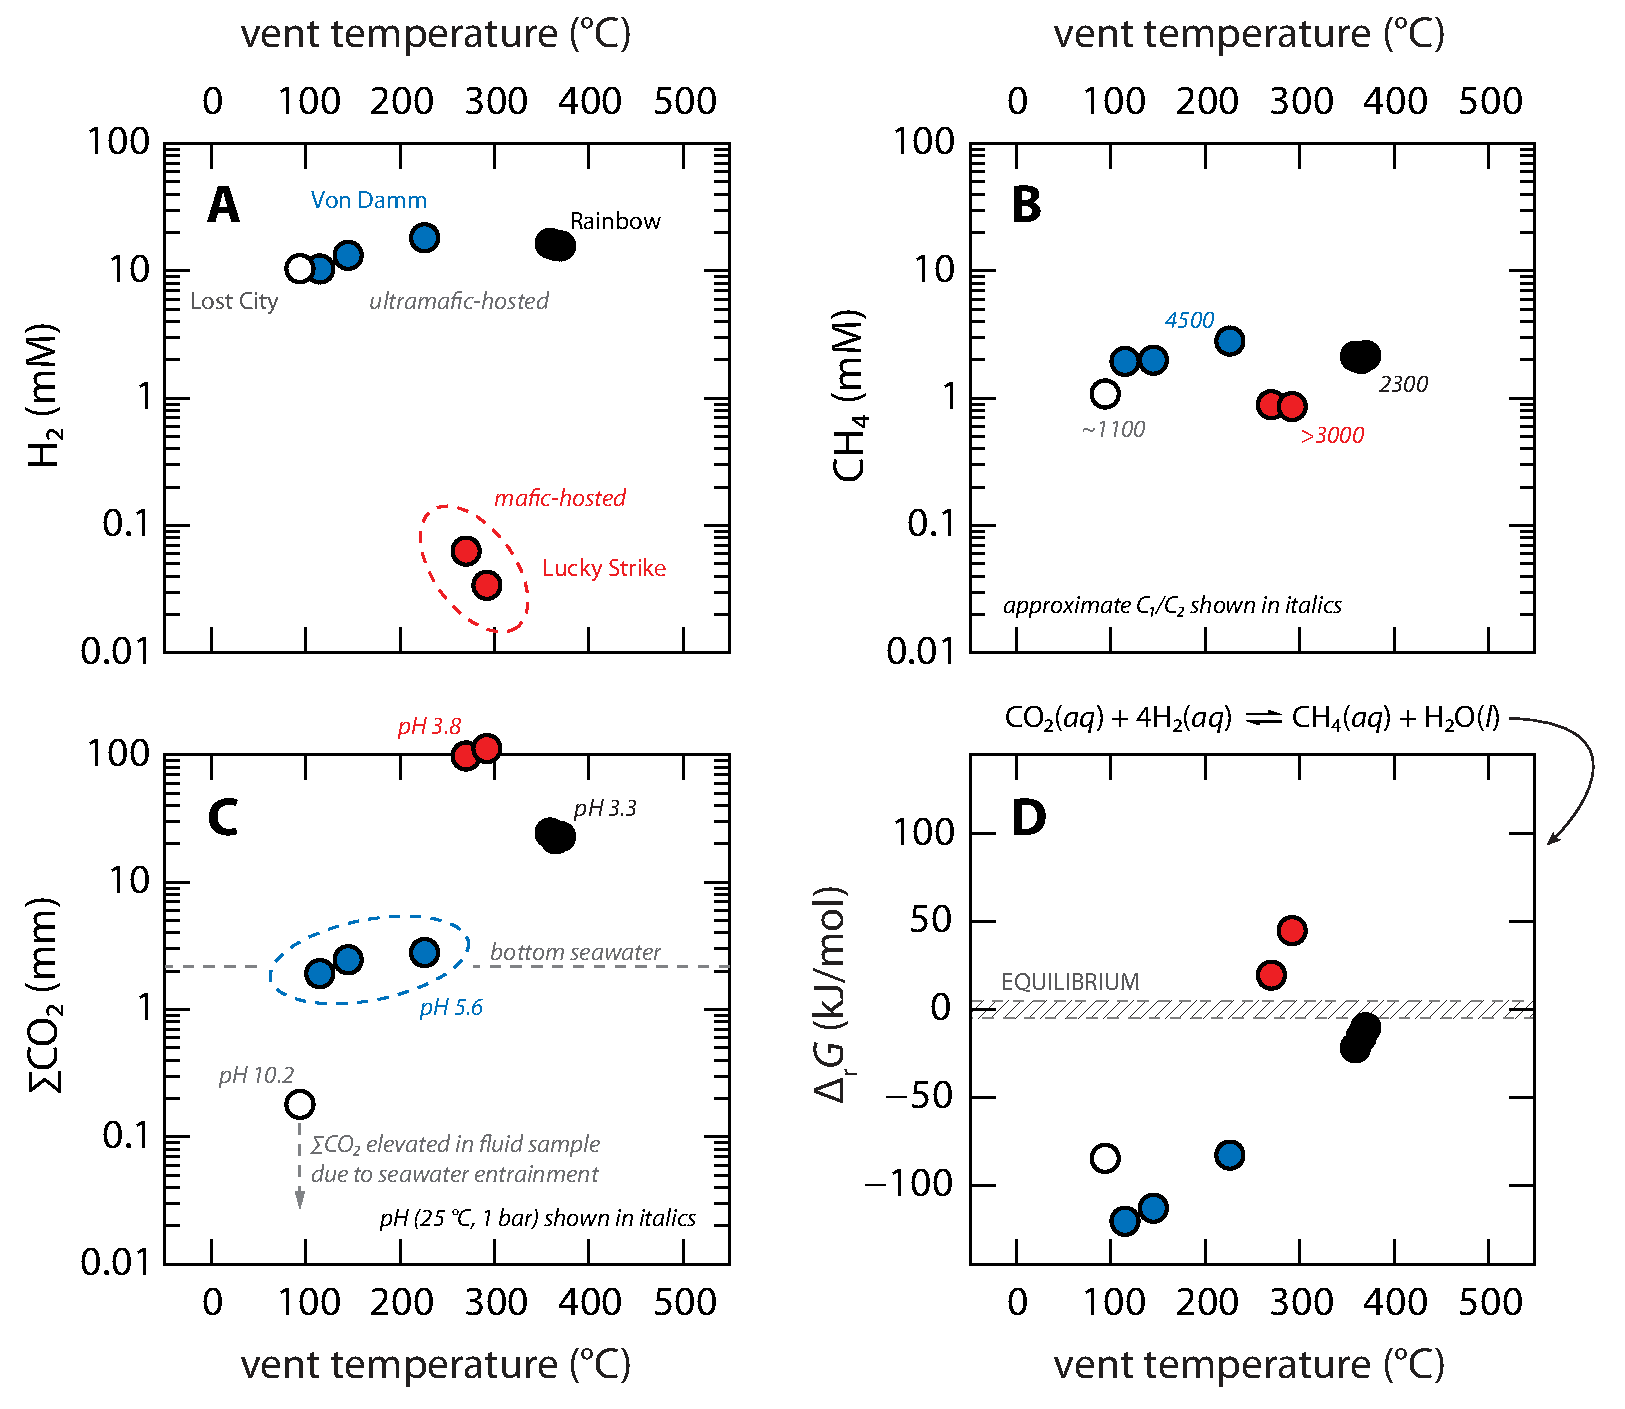
\includegraphics[width=0.95\linewidth]{figures/Fig3.3}
	\caption[Composition of vent fluids and energetics of methane synthesis in
		aqueous phase]{%
		Composition of vent fluids and energetics of methane synthesis in
		aqueous phase. Concentrations of (\textbf{A}) H\textsubscript{2},
		(\textbf{B}) CH\textsubscript{4}, and (\textbf{C}) $\big\sum\!$CO\textsubscript{2}
		are plotted against measured vent temperatures (data from \autoref{tab:3:2}). Also
		shown are molar ratios of methane to ethane
		(C\textsubscript{1}/C\textsubscript{2}, see \autoref{sec:3:results}) in (B), and pH
		values of endmember fluids in (C). (\textbf{D}) Gibbs energy of reaction
		for methane formation from CO\textsubscript{2} and H\textsubscript{2} in
		aqueous solution (\mrefs[]{Reaction}{eqn:3:2}), calculated at vent \emph{T} and \emph{P}
		conditions (Δ\textsubscript{r}\emph{G}, \autoref{tab:3:2}). Gray hatching
		represents thermodynamic equilibrium (taken as
		Δ\textsubscript{r}\emph{G} = 0 ± 5~kJ/mol). Methane formation in aqueous
		solution is thermodynamically favorable for points plotting below the
		hatched area. Symbol colors are the same as those in \mrefs[]{Figs.}{fig:3:1} and~\ref{fig:3:2}.
	}
	\label{fig:3:3}
\end{figure*}


Contents of low-molecular weight hydrocarbons are also similar between
the studied fields, with high C\textsubscript{1}/C\textsubscript{2}
ratios (\mrefs[B]{Fig.}{fig:3:3}) observed in fluids from Rainbow \parencite[\textasciitilde{}2300,][]{Charlou++_2002_CG}, Von Damm \parencite[\textasciitilde{}4500,][]{McDermott++_2015_PNAS}, Lost City \parencite[\textasciitilde{}1100,][]{Proskurowski++_2008_S}, and Lucky Strike \parencite[\textgreater{}3000,][]{Charlou++_2000_CG}. Such
high C\textsubscript{1}/C\textsubscript{2} ratios are typical of fluids
from unsedimented mid-ocean ridge hydrothermal systems \parencite{McCollom+Seewald_2007_CR}.

Except for the Lost City fluids, total dissolved inorganic carbon
($\big\sum\!$CO\textsubscript{2} = CO\textsubscript{2}(\emph{aq}) +
\(\mathrm{\text{HC}}\mathrm{O}_{\mathrm{3}}^{\mathrm{-}}\) +
\(\mathrm{C}\mathrm{O}_{\mathrm{3}}^{\mathrm{2 -}}\)) concentrations are comparable to or 
higher than CH\textsubscript{4} and are characterized by a wider range
of values (1.9 to 112.0 mmol/kg, \mrefs[C]{Fig.}{fig:3:3}). Endmember fluids from
Rainbow, Von Damm, and Lucky Strike contain 2 to 50 times as much total
carbon as is in bottom seawater \parencite[\textasciitilde{}2.2 mM;][]{McDermott++_2015_PNAS,Reeves++_2014_PNAS}, such that $\big\sum\!$CO\textsubscript{2} in
recharging seawater cannot be the sole source of carbon to venting
fluids. The Lost City fluid contains very low amounts of
$\big\sum\!$CO\textsubscript{2} (\textasciitilde{}0.18~mmol/kg), the majority of
which is likely derived from seawater entrainment during sample
collection \parencite{Reeves++_2014_PNAS}. Given the high pH (10.2), the
concentration of CO\textsubscript{2}(\emph{aq}) in endmember Lost City
fluids must be very low (see footnote~g in \autoref{tab:3:2}). At the relatively low
pH of the other fluids (3.33 to 5.81), the majority of $\big\sum\!$CO\textsubscript{2} is in the form of CO\textsubscript{2}(\emph{aq}).
%\begin{center}
\begin{table}[t]
	
	\centering
	
	\caption[Fluid compositions and Gibbs energy of reaction (Δ\textsubscript{r}\emph{G}) for
		abiotic methane formation at studied vent
		sites]{Fluid compositions\textsuperscript{a} used in thermodynamic calculations
		and calculated Gibbs energy of reaction (Δ\textsubscript{r}\emph{G}) for
		abiotic methane formation via \mrefs{Reaction}{eqn:3:2} at studied vent
		sites.\textsuperscript{b}}
	\label{tab:3:2}
	
	\begin{threeparttable}
		\small
		%\hspace*{-1ex}
		\begin{tabular}[]{@{} l l @{\!} r r r d{4} d{4} d{4} d{4} @{\!\!\!}}
			\toprule
%			{Field} & Vent & \emph{T} (°C)\textsuperscript{c} & \emph{P} (bar) & pH\textsuperscript{d} & $\big\sum\!$CO\textsubscript{2} (mm) & H\textsubscript{2} (mM) & CH\textsubscript{4} (mM) & Δ\textsubscript{r}\emph{G} (kJ/mol)\textsuperscript{e}\tabularnewline
			{Field} & Vent & \emph{T} (°C)\textsuperscript{c} & \emph{P} (bar) & pH\textsuperscript{d} & \multicolumn{1}{c}{$\big\sum\!$\ce{CO2} (mm)} & \multicolumn{1}{c}{\ce{H2} (mM)} & \multicolumn{1}{c}{\ce{CH4} (mM)} & \multicolumn{1}{c}{$\Delta_\text{r}G$ (kJ/mol)\textsuperscript{e}}\tabularnewline
			\midrule
			{Rainbow} & Guillaume & 361 & 230 & 3.33 & 24.3 & 16.5 & 2.13 & 
			-22\tabularnewline
			& CMSP\&P & 365 & 230 & 3.36 & 21.9 & 15.9 & 2.05 & -16\tabularnewline
			& Auberge & 370 & 230 & 3.35 & 22.8 & 15.7 & 2.16 & -11\tabularnewline
			{Von Damm} & Old Man Tree\textsuperscript{f} & 115 & 235 & 5.81 &
			1.80 & 10.5 & 1.97 & -121\tabularnewline
			& Ravelin 1\textsuperscript{f} & 145 & 235 & 5.83 & 2.52 & 13.4 & 2.02 &
			-113\tabularnewline
			& East Summit & 226 & 235 & 5.56 & 2.80 & 18.2 & 2.81 &
			-83\tabularnewline
			{Lost City} & Beehive & 96 & 70 & 10.20 & 0.18\textsuperscript{g}
			& 10.4 & 1.08 & -85\tabularnewline
			{Lucky Strike} & Medea & 270 & 170 & 3.81 & 98.0 & 0.063 & 0.89 &
			+20\tabularnewline
			& Isabel & 292 & 170 & 3.81 & 112.0 & 0.034 & 0.86 & +45\tabularnewline
			\bottomrule
		\end{tabular}
		%\hspace*{-1ex}	
		\begin{tablenotes}
			\item Analytical uncertainties (2\emph{s}) are ±2~°C for \emph{T}; ±5\% for
			H\textsubscript{2}, $\big\sum\!$CO\textsubscript{2}, and CH\textsubscript{4}; and
			±0.05 units for pH. Abbreviations: mm, mmol/kg fluid; mM, mmol/L fluid.
			
			\item \textsuperscript{a} All concentrations shown are extrapolated to
			endmember fluid composition (regressed to zero Mg content), except where
			noted. Data are from \textcite{McDermott++_2015_PNAS,Reeves++_2014_PNAS}.
			
			\item \textsuperscript{b} For each vent fluid, the energetic favorability of
			methane formation via this reaction was assessed by calculating the
			Gibbs energy of reaction (Δ\textsubscript{r}\emph{G}), defined by the
			relationship: Δ\textsubscript{r}\emph{G} = \emph{RT}
			ln(\emph{Q}/\emph{K}), where \emph{R} is the universal gas constant,
			\emph{T} is measured fluid temperature in kelvin, \emph{Q} is the
			reaction quotient, and \emph{K} is the equilibrium constant at \emph{T}
			and seafloor pressure \emph{P}. Equilibrium constants were calculated
			using thermodynamic data and standard states from \textcite{Johnson++_1992_CnG,Shock+Helgeson_1990_GCA}. For all calculations, the activity of
			H\textsubscript{2}O(\emph{l}) was assumed to be unity. Activity
			coefficients were assumed to be unity for neutral dissolved species. For
			all fluids except for that from Lost City,\textsuperscript{g} the
			concentration of CO\textsubscript{2}(\emph{aq}) was assumed to be equal
			to $\big\sum\!$CO\textsubscript{2}, a reasonable approximation given the low
			measured shipboard pH values and calculated equilibrium speciation of
			dissolved carbonate species at \emph{in situ} temperatures and seafloor
			pressures.
			
			\item \textsuperscript{c} Maximum measured vent temperature.
			
			\item \textsuperscript{d} Shipboard pH measurement (25~°C and 1 atm).
			
			\item \textsuperscript{e} A negative value of Δ\textsubscript{r}\emph{G}
			indicates a thermodynamic drive for the reaction to proceed as written
			from left to right (i.e., methane formation favored). Given
			uncertainties associated with chemical analyses and thermodynamic data,
			calculated Δ\textsubscript{r}\emph{G} values within ±5 kJ/mol of zero
			are interpreted to indicate that the reaction has approached or attained
			a state of thermodynamic equilibrium \parencite{Seewald_2001_GCA_minerals}.
			
			\item \textsuperscript{f} Concentrations for fluids from Old Man Tree and
			Ravelin 1 at Von Damm not extrapolated to zero Mg; Mg contents for these
			fluids are 14.0 and 15.0 mmol/kg fluid, respectively, indicating that
			endmember fluid has already mixed with seawater in the subsurface prior
			to discharge at the seafloor \parencite{McDermott++_2015_PNAS}.
			
			\item \textsuperscript{g} An arbitrary CO\textsubscript{2}(\emph{aq})
			concentration of 1 nmol/kg was used in thermodynamic calculations for
			the Lost City fluid, similar to \textcite{Reeves++_2014_PNAS}. The actual
			concentration value is subject to substantial uncertainty due to
			difficulties in determining the near-zero endmember $\big\sum\!$CO\textsubscript{2}
			content in vent fluids, given that some entrainment of
			$\big\sum\!$CO\textsubscript{2}-replete seawater always occurs during sampling
			\parencite{Proskurowski++_2008_S}. Varying this value by as much as ten orders
			of magnitude would not affect the conclusion that methane formation is
			thermodynamically favorable in the fluid, due to the high
			H\textsubscript{2} content and the power of 4 to which the activity of
			H\textsubscript{2}(\emph{aq}) is raised in the mass action expression.
	

		\end{tablenotes}

	\end{threeparttable}

\end{table}
%\end{center}

The concentration of dissolved H\textsubscript{2} is high and varies
from 10.4 to 18.2 mM in endmember and mixed fluids from the Rainbow, Von
Damm, and Lost City fields, whereas fluids from Lucky Strike have
approximately three orders of magnitude lower concentrations (34--63~µM,
\mrefs[A]{Fig.}{fig:3:3}). At Rainbow, Von Damm, and Lost City, serpentinization of
ultramafic rock in subsurface reaction zones with concomitant production
of H\textsubscript{2} is thought to be a major control on fluid
compositions \parencite{Kelley++_2001_N,Charlou++_2002_CG,McDermott++_2015_PNAS}. In contrast, the Lucky Strike field is hosted in basaltic
rock, and vent fluids there encounter much more oxidizing conditions \parencite{Charlou++_2000_CG,Pester++_2012_GCA}.

The stoichiometry of the reaction
\begin{equation}\label{eqn:3:2}
\ce{CO2\text{(\emph{aq})}} + 4\ce{H2\text{(\emph{aq})}} \leftrightharpoons
\ce{CH4\text{(\emph{aq})}} + 2\ce{H2O\text{(\emph{l})}}
\end{equation}
indicates that the abundance of CH\textsubscript{4}(\emph{aq}) at
thermodynamic equilibrium in vent fluids should be highly sensitive to
the concentration of H\textsubscript{2} because of the fourth-power
dependence on the activity of H\textsubscript{2}(\emph{aq}) in the
corresponding mass action expression. At Lucky Strike, formation of
CH\textsubscript{4}(\emph{aq}) in endmember fluids is thermodynamically
disfavored due to the low H\textsubscript{2} contents (\autoref{tab:3:2}). In all
other vent fluids studied, a thermodynamic drive for methane synthesis
is present at varying magnitudes (\mrefs[D]{Fig.}{fig:3:3}).

Methane \textsuperscript{13}C/\textsuperscript{12}C and D/H ratios are
similar across fluids from all four unsedimented hydrothermal fields
studied (\autoref{fig:3:1}). The δ\textsuperscript{13}C values ($-$18‰ to $-$11‰) are
within the range of those determined for methane at more than a dozen
other basalt- and ultramafic-hosted submarine hydrothermal systems
studied to date ($-$24‰ to $-$6‰), including Kairei on the Central Indian
Ridge, TAG, Broken Spur, and Logatchev on the Mid-Atlantic Ridge, and
17--19°S, 9°50$'$N, 13°N, and 21°N on the East Pacific Rise \parencite[see][and references therein]{Keir_2010_GRL,McCollom+Seewald_2007_CR}. Published
data for δD of methane are more limited; however, the δD values we
measured ($-$127‰ to $-$98‰) are similar to those determined at Logatchev \parencite[$-$109‰][]{Proskurowski++_2006_CG}  and 21°N on the East Pacific Rise \parencite[$-$126‰ to $-$102‰][]{Welhan+Craig_1983}.
\renewcommand{\textfraction}{0.1}  	% How much text there must be at bottom of float https://tex.stackexchange.com/a/39020
\renewcommand{\floatpagefraction}{0.9}	% only pages with more than 80% of floats, will become pure float-only pages. The default is 0.6

The data described above support the general consensus that the methane
in the studied hydrothermal fluids is of dominantly abiotic origin \parencite[e.g.,][]{Charlou++_2002_CG,McDermott++_2015_PNAS,Proskurowski++_2008_S,Welhan_1988_CG}, and that contributions of thermogenic or
microbial sources of methane are limited or insignificant. Because the
four sites studied lack substantial sediment burdens, organic carbon
from which thermogenic hydrocarbons or microbial methane can be
generated is in scarce supply \parencite{Welhan_1988_CG,Reeves++_2014_PNAS}.
Furthermore, high C\textsubscript{1}/C\textsubscript{2} ratios
(\textasciitilde{}1000 to 4000), along with high methane
δ\textsuperscript{13}C values ($-$18‰ to $-$11‰), are distinct from
thermogenic or microbial sources, which typically have lower
C\textsubscript{1}/C\textsubscript{2} ratios or lower
δ\textsuperscript{13}C values, respectively \parencite{McCollom+Seewald_2007_CR}.

The methane δ\textsuperscript{13}C data alone do not unambiguously
exclude contributions of microbial methanogenesis, because high methane
δ\textsuperscript{13}C values could be a result of near-quantitative
conversion of $\big\sum\!$CO\textsubscript{2} to CH\textsubscript{4}, particularly
under $\big\sum\!$CO\textsubscript{2}-limited and/or high-pressure conditions such as those present at
Lost City \parencite{Brazelton++_2006_AEM,Bradley+Summons_2010_EPSL,Takai++_2008_PNAS}. However,
radiocarbon (\textsuperscript{14}C) abundances for methane from Lost
City and Von Damm are very low {[}fraction modern
(\emph{F}\textsubscript{m}) averaging 0.004--0.006, near the limit of
detection (\emph{F}\textsubscript{m} \textasciitilde{} 0.003){]}
\parencite{Proskurowski++_2008_S,McDermott++_2015_PNAS}, whereas
\textsuperscript{14}C contents of endmember $\big\sum\!$CO\textsubscript{2} at Von
Damm are \textasciitilde{}5× higher \parencite{McDermott++_2015_PNAS}. Had
CH\textsubscript{4} been derived from reduction of $\big\sum\!$CO\textsubscript{2},
the younger \textsuperscript{14}C age of the $\big\sum\!$CO\textsubscript{2} would
have been transferred to CH\textsubscript{4}. \textcite{McDermott++_2015_PNAS}
further showed that $\big\sum\!$CO\textsubscript{2} in the vent fluids at Von Damm
is likely seawater-derived, because both concentrations and
δ\textsuperscript{13}C values of endmember $\big\sum\!$CO\textsubscript{2} match
those of local bottom seawater. The apparent conservation of
$\big\sum\!$CO\textsubscript{2} during convective circulation at Von Damm indicates
that $\big\sum\!$CO\textsubscript{2} in recharging seawater at Von Damm has not
been converted to CH\textsubscript{4} via any process---microbial or
otherwise---despite high energetic favorability for CH­\textsubscript{4}
synthesis (\mrefs[D]{Fig.}{fig:3:3}). Similar carbon isotopic compositions of
CH\textsubscript{4} and contents of C\textsubscript{2+} alkanes at Lost
City, Lucky Strike, and Rainbow (as well as at other unsedimented fields
studied to date), despite marked differences in geologic setting, fluid
composition, and thermodynamic drive for CH\textsubscript{4} synthesis,
are consistent with a common abiotic origin for methane at many, if not
all, sediment-poor seafloor hydrothermal systems.
\begin{SCfigure*}
	\centering
	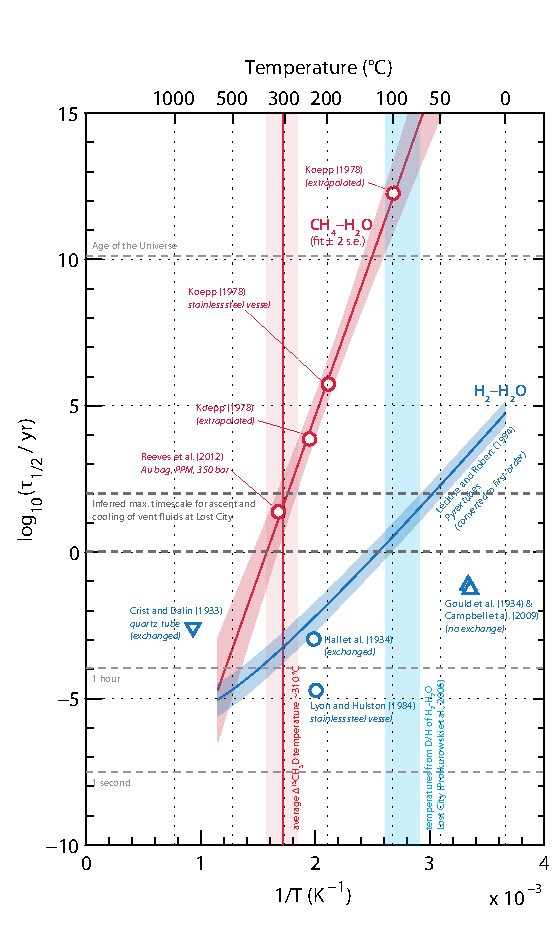
\includegraphics[width=0.625\linewidth]{figures/Fig3.4}
	\caption[Half-exchange timescales for hydrogen exchange between CH\textsubscript{4} \& H\textsubscript{2}O
 and H\textsubscript{2} \& H\textsubscript{2}O ]{%
		Half-exchange time\-scales ($\tau_{1/2} = \ln(2)/k$) for
		hydro\-gen exchange between CH\textsubscript{4} \& H\textsubscript{2}O
		(red sym\-bols) and H\textsubscript{2} \& H\textsubscript{2}O (blue) based
		on experiments done in the absence of added catalyst
		\parencite{Crist+Dalin_1933_JCP,Hall++_1934_JACS,Gould++_1934_JCP,Koepp_1978,Lyon+Hulston_1984_GCA,Lecluse+Robert_1994_GCA,Campbell++_2009_GCA,Reeves++_2012_GCA}.
	 	Reactions were assumed to be first order in
		CH\textsubscript{4} or H\textsubscript{2}. When rate constants were not
		provided by the authors or when exchange was not observed, the reported
		duration of the experiment was taken as an estimate of the timescale of
		exchange. Downward- and upward-pointing triangles are, respectively,
		maximum and minimum estimates of the exchange timescale. The
		$\tau_{1/2}$ for CH\textsubscript{4}--H\textsubscript{2}O
		exchange from \textcite{Reeves++_2012_GCA} comes from \autoref{fig:3:S2}.
		Second-order rate coefficients for
		H\textsubscript{2}--H\textsubscript{2}O exchange from \textcite{Lecluse+Robert_1994_GCA} were converted to first-order rate coefficients by multiplying by
		the equilibrium vapor pressure of H\textsubscript{2}O calculated at
		temperatures \emph{T} and a pressure of 1~kbar. Uncertainties in
		exchange rates are difficult to estimate, but are probably one order of
		magnitude or greater. Clumped isotopologue temperatures for
		CH\textsubscript{4} from the present study (red bar) and temperatures
		from D/H geothermometry of H\textsubscript{2}--H\textsubscript{2}O in
		endmember fluids at the Lost City site (blue bar) \parencite{Proskurowski++_2006_CG} are also shown. See text for interpretation of these data with
		respect to timescales of fluid circulation.
	}
	\label{fig:3:4}
\end{SCfigure*}

Measured Δ\textsuperscript{13}CH\textsubscript{3}D values (averaging
1.57 ± 0.28‰, 1\emph{s}) and corresponding apparent equilibrium
temperatures (\(310_{- 42}^{+ 53}\)~°C) are strikingly uniform in the
context of the large natural variations (up to ca.\ 10‰) previously
observed in Δ\textsuperscript{13}CH\textsubscript{3}D values carried by
methane sampled from different settings \parencite{Wang++_2015_S}.
Furthermore, the studied fluids vented at a wide range of temperatures,
ranging from 96 to 370~°C. Had the methane in these samples attained
isotopologue equilibrium at measured vent temperatures,
Δ\textsuperscript{13}CH\textsubscript{3}D values from 4.0 to 1.3‰,
respectively, would be expected. The observed range of clumped
isotopologue data is much smaller than this predicted range (\mrefs[C]{Fig.}{fig:3:1}),
with Δ\textsuperscript{13}CH\textsubscript{3}D temperatures generally
equal to or higher than fluid temperatures (\mrefs[B]{Fig.}{fig:3:2}). In
lower-temperature (\textless{}250~°C) fluids, including fluids that have
mixed in the subsurface (venting with non-zero Mg) such as those from
Ravelin 1 (145~°C) and Old Man Tree (115~°C) vents at Von Damm
\parencite{McDermott++_2015_PNAS}, Δ\textsuperscript{13}CH\textsubscript{3}D
temperatures higher than fluid temperatures indicate that
Δ\textsuperscript{13}CH\textsubscript{3}D values have not been affected
by cooling below \textasciitilde{}250~°C. In higher temperature fluids
(\textgreater{}270~°C) however,
Δ\textsuperscript{13}CH\textsubscript{3}D temperatures are analytically
indistinguishable from measured fluid temperatures. Experimental data
suggest that hydrogen exchange between methane and water in hydrothermal
fluids may be observable at temperatures of \textasciitilde{}325~°C on
relatively short timescales \parencite[years;][and \autoref{fig:3:S2}]{Reeves++_2012_GCA}
relevant to hydrothermal systems (\autoref{fig:3:4}). Hydrogen exchange between
CH\textsubscript{4} and H\textsubscript{2}O may explain the uniformity
of both δD and Δ\textsuperscript{13}CH\textsubscript{3}D values of
methane in high-temperature fluids (\autoref{fig:3:5}); the implications of this
are discussed below (\autoref{hydrogen-exchange-and-the-origin-of-hydrogen-in-ch4}). The
Δ\textsuperscript{13}CH\textsubscript{3}D values indicate that
CH\textsubscript{4} experienced temperatures of at least 300~°C during
its residence within the oceanic crust. Our methane clumped isotopologue
data indicate that temperatures and compositions of hot-spring fluids at
the time of venting are decoupled from the conditions responsible for
the formation of CH\textsubscript{4} in these fluids. The following
sections discuss how the 300~°C or greater inferred temperatures are
compatible with models invoking respeciation of magmatic volatiles at
those temperatures to form CH\textsubscript{4} in plutonic layers of the
oceanic crust.

\subsection{\texorpdfstring{Hydrogen exchange and the origin of
		hydrogen in
		CH\textsubscript{4}}{Hydrogen exchange and the origin of hydrogen in CH4}}\label{hydrogen-exchange-and-the-origin-of-hydrogen-in-ch4}

Hydrogen isotope ratio measurements provide constraints on the origin of
the major H-bearing species within vent fluids. Apparent temperatures
derived from D/H equilibria in the systems
H\textsubscript{2}--H\textsubscript{2}O and
H\textsubscript{2}--CH\textsubscript{4} were first used as
geothermometers in studies of geothermal or volcanic gases and waters
\parencite{Arnason_1977_Geothermics,Arnason+Sigurgeirsson_1968_GCA,Gunter+Musgrave_1971_GCA,Panichi++_1977_Geothermics,Panichi+Gonfiantini_1977_Geothermics,Kiyosu_1983_EPSL,Lyon+Hulston_1984_GCA}, and later examined with respect to data from
seafloor hydrothermal fluids \parencite{Welhan+Craig_1983,Horibe+Craig_1995_GCA,Proskurowski++_2006_CG,Bradley+Summons_2010_EPSL,Kawagucci++_2010_JGR,Kawagucci++_2011_GcJ,Kawagucci++_2013_CG}, shield-hosted groundwaters
\parencite{SherwoodLollar++_1993_GCA_abiogenic,SherwoodLollar++_2007_Ab,SherwoodLollar++_2008_GCA}, and continental
springs, seeps, and well fluids influenced by serpentinization \parencite{Fritz++_1992,Neal+Stanger_1983_EPSL,Coveney++_1987_AAPGB,Abrajano++_1988_CG,Etiope++_2011_CG,Suda++_2014_EPSL}. Temperatures returned from
H\textsubscript{2}--H\textsubscript{2}O and
H\textsubscript{2}--CH\textsubscript{4} equilibria often agree with each
other and with realistic geologic and hydrologic scenarios for
geothermal fluids exiting at high temperatures, but these relationships
do not necessarily hold for lower-temperature fluids. 

\textcite{Proskurowski++_2006_CG} showed that D/H-based temperatures derived
from H\textsubscript{2}--H\textsubscript{2}O and
H\textsubscript{2}--CH\textsubscript{4} in high-temperature vent fluids
(\textgreater{}270~°C) are concordant and match measured fluid
temperatures at discharge. At the low-temperature Lost City site,
however, H\textsubscript{2}--H\textsubscript{2}O and  
H\textsubscript{2}--CH\textsubscript{4} yielded discordant temperatures
of 70--110~°C and 110--150~°C, respectively. \textcite{Proskurowski++_2006_CG}
reconciled these data by suggesting that serpentinization of ultramafic
basement rocks beneath the Lost City vent field occurs at low
temperatures of 110--150~°C, concomitant with production of both
H\textsubscript{2} and CH\textsubscript{4}, and that H\textsubscript{2}
maintained isotopic equilibrium with H\textsubscript{2}O during slow
cooling of root-zone fluids to ca.\ 70--110~°C prior to rapid ascent to
seafloor while the higher temperature signal recorded by
H\textsubscript{2}--CH\textsubscript{4} was presumably not reset during
cooling. In contrast, the Δ\textsuperscript{13}CH\textsubscript{3}D
temperature of \(270_{- 68}^{+ 104}\)~°C we obtained for the Beehive
vent fluid argues for a much higher temperature of last exchange for the
C--H bonds in methane, and does not support suggestions of
CH\textsubscript{4} production at lower temperatures. The clumped
isotopologue temperature is consistent with estimates from heat balance
considerations, δ\textsuperscript{18}O values, and alkane-alkene and
mineral-fluid equilibria all suggesting that Lost City fluids
experienced temperatures as high as 250~°C at depth \parencite{Allen+Seyfried_2004_GCA,Foustoukos++_2008_GCA,Reeves++_2012_GCA,Seyfried++_2015_GCA}. Discrepancies between measured
Δ\textsuperscript{13}CH\textsubscript{3}D temperatures, temperatures
from D/H geothermometry, and fluid exit temperatures at Lost City
indicate that rather than directly recording the temperatures of
H\textsubscript{2} and CH\textsubscript{4} synthesis, each
geothermometer records a different portion of the time-temperature
history of the fluids.

\afterpage{%
	\clearpage
	
	\begin{landscape}
	
		\begin{figure*}[p]
			\centering
			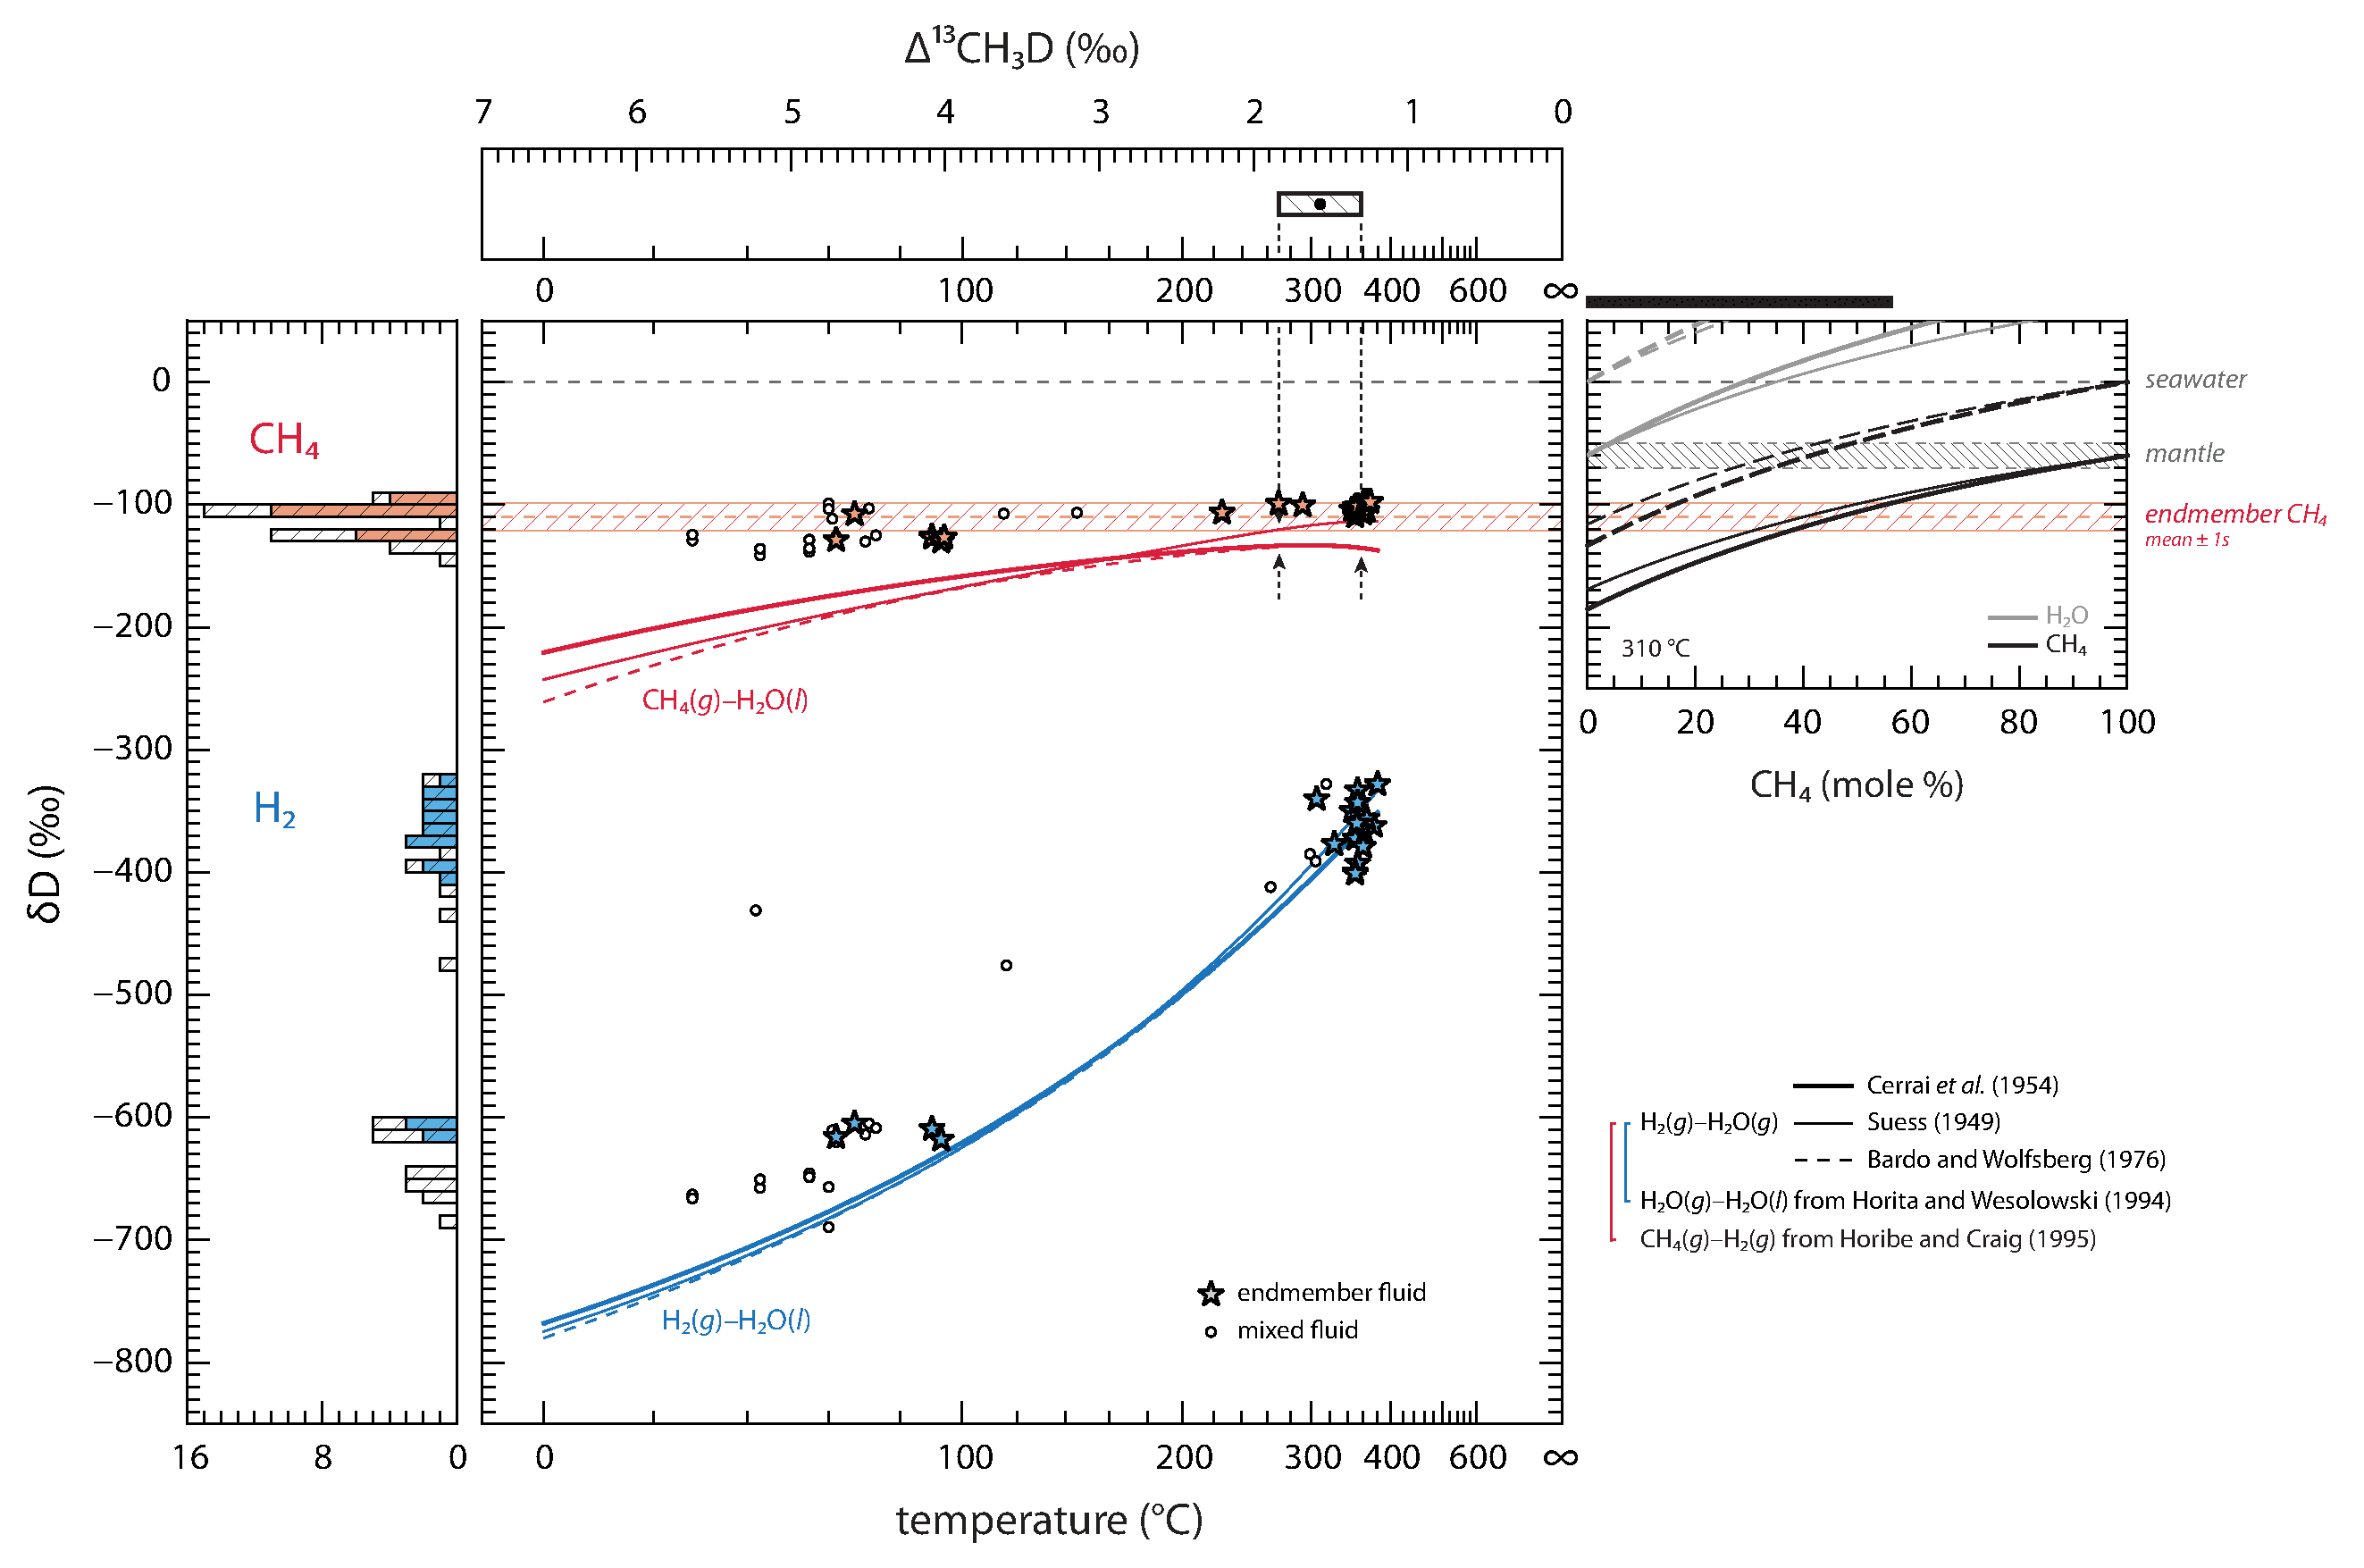
\includegraphics[width=\linewidth]{figures/Fig3.5}
			
			
			
		\end{figure*}
	
	\end{landscape}
	%\addtocounter{figure*}{-1}	% decrement counter because putting figure caption in next float
	
	\begin{landscape}
		
		\begin{figure*}[h!]
			\caption[Data and models of D/H of CH\textsubscript{4} and H\textsubscript{2} in seafloor hydrothermal fluids]{%
			Hydrogen
			isotopic composition of CH\textsubscript{4} (red) and H\textsubscript{2}
			(blue) in seafloor hydrothermal fluids plotted against measured vent
			temperatures. Data are from unsedimented fields studied in \textcite{Welhan+Craig_1983,Proskurowski++_2006_CG,Kawagucci++_2010_JGR,Charlou++_2010}, and in this study (see \mrefs[]{Tables}{tab:3:1} and~\ref{tab:3:1}), and are tabulated in
			\autoref{tab:3:S1}. Endmember fluids (identified by low Mg contents)
			are represented by stars, and vent fluids containing a mixture of
			hydrothermal endmember fluid and seawater are represented by circles.
			Data from sites exhibiting phase separation \parencite{Charlou++_2010} or
			with fluids diffusely effluxing through colonies of deep-sea snails or
			shrimp \parencite{Kawagucci++_2010_JGR} are excluded from this plot (see notes
			under \autoref{tab:3:S1}). Red hatching indicates the average δD of
			CH\textsubscript{4} in endmember fluids ($-$110 ± 12‰, 1\emph{s}) in the
			compiled dataset. Red and blue curves represent the δD values of
			CH\textsubscript{4} and H\textsubscript{2} (respectively) in D/H
			equilibrium with H\textsubscript{2}O of seawater-like isotopic
			composition (δD = 0‰, dashed gray line) predicted by combinations of
			published calibrations for
			H\textsubscript{2}(\emph{g})/H\textsubscript{2}O(\emph{g}) \parencite{Suess_1949,Cerrai++_1954,Bardo+Wolfsberg_1976_JPC},
			H\textsubscript{2}O(\emph{g})/H\textsubscript{2}O(\emph{l}) \parencite{Horita+Wesolowski_1994_GCA}, and
			CH\textsubscript{4}(\emph{g})/H\textsubscript{2}(\emph{g}) \parencite{Horibe+Craig_1995_GCA}. {[}High-temperature hydrothermal fluids generally have δD
			values of H\textsubscript{2}O close to 0‰ \parencite{Shanks++_1995_AGU-GM}. Note
			that measured values for δD of H\textsubscript{2}O in fluids from Lost
			City are +2 to +7‰ \parencite{Proskurowski++_2006_CG} and thus the equilibrium
			values for CH\textsubscript{4} and H\textsubscript{2} at Lost City are
			slightly (\textasciitilde{}5‰) higher than those indicated by the
			curves; this difference is small compared to the uncertainty in
			equilibrium fractionation factor calibrations at the temperatures of
			these fluids (\textasciitilde{}30 to 90~°C).{]} (\emph{\textbf{Left}})
			Histogram of δD values of CH\textsubscript{4} and H\textsubscript{2} in
			endmember (shaded) and mixed fluids (unshaded bars).
			(\emph{\textbf{Top}}) Mean ± 1\emph{s} of the
			Δ\textsuperscript{13}CH\textsubscript{3}D values and corresponding
			clumped isotopologue temperatures (\(310_{- 42}^{+ 53}\)~°C) of methane
			reported in \autoref{tab:3:1}. Dashed black arrows point to the range of δD values
			of CH\textsubscript{4}(\emph{g}) in equilibrium with seawater at the
			temperatures indicated by Δ\textsuperscript{13}CH\textsubscript{3}D
			data. (\emph{\textbf{Right}}) Modeled δD values of CH\textsubscript{4}
			(black curves) and H\textsubscript{2}O (gray curves) as a function of
			mole fraction of CH\textsubscript{4} in a hypothetical methane-rich
			fluid. All H was assumed to exist as H\textsubscript{2}O(\emph{l}) in
			isotopic equilibrium with CH\textsubscript{4}(\emph{g}) at the
			temperature indicated by the mean
			Δ\textsuperscript{13}CH\textsubscript{3}D value (310~°C). {[}At
			\textasciitilde{}270 to 360~°C, D/H fractionation between
			CH\textsubscript{4}(\emph{g}) and H\textsubscript{2}O(\emph{l}) is not
			very sensitive to temperature \parencite{Horibe+Craig_1995_GCA}. Uncertainty in
			the equilibrium D/H fractionation factor is dominated by the
			disagreement among
			H\textsubscript{2}(\emph{g})/H\textsubscript{2}O(\emph{g}) calibrations.
			Isotopic fractionation between CH\textsubscript{4}(\emph{g}) and
			CH\textsubscript{4}(\emph{aq}) is negligible \parencite{Bacsik++_2002_JCP}, and
			the fractionation between H\textsubscript{2}O(\emph{g}) and
			H\textsubscript{2}O(\emph{l}) is small (\textasciitilde{}5‰) \parencite{Horita+Wesolowski_1994_GCA}. The model neglects the effects of elevated pressure
			and salinity \parencite{Horita_2005_GcJ,Martineau++_2012_CG}, and ignores
			potential isotopic exchange with hydrous minerals \parencite{Horita++_1999_S,Saccocia++_2009_GCA,Meheut++_2010_GCA}.{]} The initial δD was taken
			to be 0‰ (dashed lines) for seawater-derived H, or $-$60‰ (solid lines)
			for mantle-derived H \parencite{Clog++_2013_EPSL}. Minimum and maximum values
			expected for δD of CH\textsubscript{4} are represented by the solid and
			dashed lines, respectively. Mixing of seawater with mantle-derived water
			prior to respeciation of H\textsubscript{2}O to CH\textsubscript{4} and
			re-equilibration of CH\textsubscript{4} initially formed in equilibrium
			with mantle-derived H\textsubscript{2}O (both resulting in δD values of
			CH\textsubscript{4} moving upwards towards the dashed lines) affect the
			predictions; effects of these processes are treated in \autoref{sec:3:discussion}. The black bar shows the range in CH\textsubscript{4}
			mole fraction that is compatible with the isotopic data from vent
			fluids.
		}
		\label{fig:3:5}
	\end{figure*}
	
	\clearpage
}

\end{landscape} 

Comparison of temperatures indicated by these
H\textsubscript{2}--H\textsubscript{2}O and
H\textsubscript{2}--CH\textsubscript{4} geothermometers are only
meaningful if H\textsubscript{2}--H\textsubscript{2}O,
H\textsubscript{2}--CH\textsubscript{4}, and
CH\textsubscript{4}--H\textsubscript{2}O have all attained equilibrium
at a single temperature, and no further isotopic exchange has occurred
during cooling. These temperatures cannot be considered in isolation
because a shift in the D/H ratio of one species induces disequilibrium
in two of the three reactions. Stated another way, the inferences drawn
by \textcite{Proskurowski++_2006_CG} implicitly required that hydrogen exchange
processes among H\textsubscript{2}O, H\textsubscript{2}, and
CH\textsubscript{4} have similar kinetics and closure temperatures.
This assumption may not hold at temperatures \textless{}300~°C. In
particular, H\textsubscript{2}--H\textsubscript{2}O exchange occurs at
substantially higher rates than does
CH\textsubscript{4}--H\textsubscript{2}O \parencite{Lyon+Hulston_1984_GCA,Lecluse+Robert_1994_GCA,Horibe+Craig_1995_GCA}. In \autoref{fig:3:4}, we show
timescales for exchange at temperatures between 0 and 600~°C, determined
from published data for experimental isotopic exchange in the systems
CH\textsubscript{4}--H\textsubscript{2}O and
H\textsubscript{2}--H\textsubscript{2}O. This compilation indicates that
although the exact rate of exchange is highly uncertain,
H\textsubscript{2}--H\textsubscript{2}O exchange occurs much faster than
CH\textsubscript{4}--H\textsubscript{2}O exchange. The rate coefficients
of \textcite{Lecluse+Robert_1994_GCA} were obtained in vapor-phase experiments
where H\textsubscript{2} was exchanged with D\textsubscript{2}O. They
observed no discernible difference in rates of exchange when several
different catalysts were added to increase available surface area for
reaction. The plotted blue curve shows their data converted to rates
that are first-order in {[}H\textsubscript{2}{]}; whether the converted
rate coefficients accurately reflect real kinetics of
H\textsubscript{2}--H\textsubscript{2}O exchange where
H\textsubscript{2} is dissolved in liquid H\textsubscript{2}O remains to
be evaluated. \textcite{Lyon+Hulston_1984_GCA} reported D/H exchange of
H\textsubscript{2} with liquid H\textsubscript{2}O on timescales of
\textasciitilde{}10 minutes at 225~°C in a stainless steel reaction
vessel. Their rate is faster than those we calculated from the data of
\textcite{Lecluse+Robert_1994_GCA}, suggesting either that rates of
H\textsubscript{2}--H\textsubscript{2}O exchange may be faster than
projected by the blue curve, or that catalytic effects of stainless
steel enhanced rates of exchange in \citeauthor{Lyon+Hulston_1984_GCA}'s experiment. In
comparison to the H\textsubscript{2}--H\textsubscript{2}O data, the
experimental data for CH\textsubscript{4}--H\textsubscript{2}O exchange
(red symbols in \autoref{fig:3:4}) provide a surprisingly good fit, though
alignment of the limited data could be fortuitous. However, the
experiments of \textcite{Reeves++_2012_GCA} were conducted in a gold-titanium
reaction cell in the presence of mineral phases typical of those found
in hydrothermal deposits, and may simulate natural conditions fairly
well. It is not known if factors such as pH, redox state, minerals, or
concentrations of sulfur, H\textsubscript{2}, or carbon species affect
hydrogen exchange rates. Regardless,
CH\textsubscript{4}--H\textsubscript{2}O exchange is at least several
orders of magnitude slower than H\textsubscript{2}--H\textsubscript{2}O
exchange.
\renewcommand{\textfraction}{0.2}
\renewcommand{\floatpagefraction}{0.6}

Across many low- and high-temperature hydrothermal systems globally, δD
of H\textsubscript{2} varies systematically (between $-$700‰ and $-$330‰)
with measured fluid temperature (40 to 370~°C, respectively), whereas δD
of CH\textsubscript{4} falls within a much narrower range ($-$140‰ to
$-$95‰) and shows no correlation with fluid temperature (\autoref{fig:3:5}). Within
the Lost City site, δD of H\textsubscript{2} varies by up to 80‰ while
δD of CH\textsubscript{4} shows much less variation (a 40‰ range)
\parencite{Proskurowski++_2006_CG}.\footnotemark{} 
\footnotetext{At lower-temperature vents,
	isotopic compositions of CH\textsubscript{4} may reflect admixture or
	removal of minor amounts of CH\textsubscript{4} due to biological
	activity \parencite{Brazelton++_2006_AEM,Proskurowski++_2006_CG,Bradley+Summons_2010_EPSL}.}
Hydrogen-isotope ratio data of H\textsubscript{2}--CH\textsubscript{4} here 
indicate spurious temperatures that do not reflect recent exchange 
between these two species.\footnotemark{} 
\footnotetext{While rates of D/H exchange between dissolved
	H\textsubscript{2} and CH\textsubscript{4} have not been
	experimentally studied, the discordant temperatures from D/H
	geothermometry in low-temperature fluids (described above) strongly
	suggest that direct H\textsubscript{2}--CH\textsubscript{4} exchange
	is also much slower than H\textsubscript{2}--H\textsubscript{2}O
	exchange.}
Part of the problem is that H\textsubscript{2}--CH\textsubscript{4} will always give a temperature
that is close to H\textsubscript{2}--H\textsubscript{2}O if δD of
H\textsubscript{2}O and CH\textsubscript{4} are within a few hundred
permil because the δD of H\textsubscript{2} directly controls the
calculated temperature for both. This means that temperatures derived
from H\textsubscript{2}--CH\textsubscript{4} may not be meaningful
unless they can be confirmed by something else such as clumped isotopes.
Decoupling of D/H data of CH\textsubscript{4} from H\textsubscript{2} at
Lost City suggests that these species have not recently interacted with
each other, and are more appropriately interpreted as recording separate
temperatures at which these species independently equilibrated with
water (H\textsubscript{2} at \textasciitilde{}110~°C in endmember
fluids, and CH\textsubscript{4} at much higher temperatures of
\textgreater{}240~°C). An origin of CH\textsubscript{4} that is
separated in time, space and/or temperature from that of
H\textsubscript{2} is compatible with the fluid inclusion-leaching
hypothesis (\autoref{magmatic-volatiles-in-the-oceanic-crust-and-the-origin-of-carbon-in-ch4}) and is corroborated by our
Δ\textsuperscript{13}CH\textsubscript{3}D data.

 \addtocounter{footnote}{-2} 	% n = 2
 \stepcounter{footnote}
 \stepcounter{footnote}

Given the rate of CH\textsubscript{4}--H\textsubscript{2}O isotope
exchange of 10 to 100~years at 300~°C (\autoref{fig:3:4}), it is likely that the
clumped methane isotopologue temperatures represent closure
temperatures below which exchange becomes sluggish relative to cooling
rate. The δD values of methane might constrain the source of water with
which CH\textsubscript{4} equilibrated at that temperature. Measured δD values of
CH\textsubscript{4} ($-$149 to $-$99‰) and H\textsubscript{2}O ($-$104 to $-$6‰)
in the gabbro-hosted inclusions from the Southwest Indian Ridge \parencite{Kelley+FruhGreen_1999_JGR} are consistent with predictions from a model of a
fluid containing mantle-derived H that partitioned into
CH\textsubscript{4} and H\textsubscript{2}O at \textasciitilde{}310~°C
(\autoref{fig:3:5}). The δD values of CH\textsubscript{4} in the inclusions overlap
the observed ranges in vent fluids shown in \autoref{fig:3:5} and \autoref{tab:3:S1} ($-$141 to $-$93‰). Partial or total re-equilibration of C--H bonds
in CH\textsubscript{4} during extraction by seawater heated to
\textgreater{}300~°C during active hydrothermal circulation would pull
the δD values of CH\textsubscript{4} towards an equilibrium value of
$-$130 to $-$110‰ (depending on the calibration), consistent with the narrow
range of data from high-temperature endmember fluids (\autoref{fig:3:5}).

It is worth noting that while serpentinization of olivine and
orthopyroxene in oceanic peridotites generates large quantities of
H\textsubscript{2} \parencite{Klein++_2009_GCA,McCollom+Bach_2009_GCA,Klein++_2013_L}, methane synthesis does not necessarily require
serpentinization of peridotite. At temperatures of
\textasciitilde{}400~°C, oxygen fugacities at or below FMQ are
sufficiently reducing for CH\textsubscript{4} to be stable relative to
CO\textsubscript{2} (\mrefs[]{Figs.}{fig:3:2} and~\ref{fig:3:S1}). Rocks derived
from the partial melting of the suboceanic upper mantle, including
gabbros and mid-ocean ridge basalts, are typically characterized by
\(f_{\mathrm{O}_{\mathrm{2}}}\) within ±1 log unit of FMQ at
temperatures and pressures of the upper mantle \parencite{Bryndzia+Wood_1990_AJS,Cottrell+Kelley_2011_EPSL}. Cooling of these rocks along an
\(f_{\mathrm{O}_{\mathrm{2}}}\) trajectory parallel to those of typical
oxygen buffers may allow for respeciation of mantle-derived
CO\textsubscript{2} to CH\textsubscript{4} to occur in the presence of
mafic minerals (olivine and orthopyroxene) deep within the oceanic crust
\parencite{Mathez++_1989_JPetrol,Kelley+FruhGreen_1999_JGR}. Serpentinization
occurring distal to the rocks from which CH\textsubscript{4}-rich fluids
are extracted may explain why CH\textsubscript{4} and H\textsubscript{2}
concentrations are not tightly correlated across seafloor hydrothermal
systems \parencite{Keir_2010_GRL,Kawagucci++_2013_CG}.

Models of convective hydrothermal circulation at Lost City indicate that
the bulk of actively-venting fluids have migrated along a narrow range
of flow paths that are surrounded by already fully-serpentinized rock
with little additional potential for H\textsubscript{2} generation,
suggesting that H\textsubscript{2} in vent fluids may have instead
formed by serpentinization occurring in meandering flow paths away from
the main flow channels, and later diffused or mixed into the ascending
fluid \parencite{Titarenko+McCaig_2016_Gf}. Assuming that equilibration of the
methane isotopologues proceeds through
CH\textsubscript{4}--H\textsubscript{2}O exchange,
Δ\textsuperscript{13}CH\textsubscript{3}D temperatures for
CH\textsubscript{4} from the present study (red bar in \autoref{fig:3:4}) suggest
that the time taken by actively-circulating hydrothermal fluids (after
extracting CH\textsubscript{4} from plutonic rocks) during ascent from
the \textasciitilde{}270~°C isotherm to temperatures below
\textasciitilde{}200~°C (at which further equilibration is no longer
possible on any relevant timescale) is
\textasciitilde{}10\textsuperscript{2}~years or less. This compares
favorably with estimates for fluid residence times in hydrothermal
systems, which generally suggest that the bulk of vent fluids in several
high-temperature systems resided in the reaction zone
(\textgreater{}200~°C) for years to decades prior to venting \parencite{Kadko_1996,Fisher_2003}. Projection onto the blue bar in \autoref{fig:3:4} showing
temperatures from D/H geothermometry of
H\textsubscript{2}--H\textsubscript{2}O in endmember fluids at Lost City
\parencite{Proskurowski++_2006_CG} shows that these timescales for fluid
transit are also consistent with estimated kinetics of D/H exchange
between H\textsubscript{2} and H\textsubscript{2}O. Timescales inferred
here may also be compared with constraints on upflow velocities from 1D
reactive transport models of fluids ascending from
\textasciitilde{}750~mbsf and cooling via conduction \parencite{Seyfried++_2015_GCA}. Actual timescales of circulating
fluid may vary widely due to significant contributions of both on- and
off-axis recharge and circulation \parencite{Hasenclever++_2014_N}.

This study emphasizes that the use of bulk and position-specific D/H
ratios and clumped isotopologues abundances of small organic molecules
as geothermometers or geospeedometers requires an understanding of the
factors controlling hydrogen exchange rates \parencite{Eiler_2013_AREarth}. Rigorous
exchange experiments under simulated natural conditions may yield
broadly-applicable insights into interactions of CH\textsubscript{4} or
other hydrocarbons with minerals or water. Substantial hydrogen isotopic
exchange of C\textsubscript{2} to C\textsubscript{5­} alkanes with
D-enriched and D-depleted water occurs during hydrothermal experiments
lasting several months at 323~°C \parencite{Reeves++_2012_GCA}. In contrast,
hydrogen exchange between CH\textsubscript{4} and H\textsubscript{2}O
proceeds much more slowly than hydrogen exchange between
C\textsubscript{2+} hydrocarbons and H\textsubscript{2}O, likely because
double-bond formation---which leads to metastable equilibrium between
alkanes and alkenes \parencite{Seewald_1994_N}---cannot occur for
CH\textsubscript{4}. Timescales determined for
CH\textsubscript{4}--H\textsubscript{2}O exchange provide a maximum
estimate of the stability of C--H bonds of organic molecules in nature,
which in turn sets bounds on the integrity of interpretations that
require δD values to be primary in origin \parencite{Sessions++_2004_GCA,Schimmelmann++_2006_AREarth}.

\subsection{\texorpdfstring{Magmatic volatiles in the oceanic crust
		and the origin of carbon in CH\textsubscript{4}
	}{Magmatic volatiles in the oceanic crust and the origin of carbon in CH4 }}\label{magmatic-volatiles-in-the-oceanic-crust-and-the-origin-of-carbon-in-ch4}

At Von Damm, constraints from δ\textsuperscript{13}C and
\textsuperscript{14}C data of $\big\sum\!$CO\textsubscript{2} and
CH\textsubscript{4} indicate that reduction of seawater-derived
$\big\sum\!$CO\textsubscript{2} to CH\textsubscript{4} is not occurring to an
appreciable extent in the actively convecting hydrothermal fluids (see
\autoref{decoupling-of-vent-fluid-chemistry-and-temperatures-from-conditions-responsible-for-ch4-synthesis}), despite the energetic favorability of reduction of
CO\textsubscript{2}(\emph{aq}) to CH\textsubscript{4}(\emph{aq})
(\mrefs[D]{Fig.}{fig:3:3}). Instead, metastable equilibrium is established between $\big\sum\!$HCOOH
(= formate + formic acid) and $\big\sum\!$CO\textsubscript{2} as a result of
kinetic limitations on CH\textsubscript{4} production \parencite{McDermott++_2015_PNAS}. \citeauthor{McDermott++_2015_PNAS} suggested that hydrocarbons here might instead
be derived from leaching of fluids occluded in plutonic rocks of the
Mount Dent oceanic core complex that originally contained magmatic
CO\textsubscript{2} and which respeciated to form hydrocarbons at
temperatures at or below 400~°C, as suggested by several studies of
gabbros from the Southwest Indian Ridge \parencite{Kelley_1996_JGR,Kelley+FruhGreen_1999_JGR}. The Δ\textsuperscript{13}CH\textsubscript{3}D
temperatures we obtained for fluids from three vents in the Von Damm
field (averaging between 288 and 350~°C, \autoref{tab:3:1}) are significantly
higher than the fluid temperatures measured at discharge (115 to 226~°C,
\mrefs[B]{Fig.}{fig:3:2}), but lower than 400~°C. The data presented here are compatible
with the inclusion-leaching hypothesis of \textcite{McDermott++_2015_PNAS}.


\begin{SCfigure*}
	\centering
	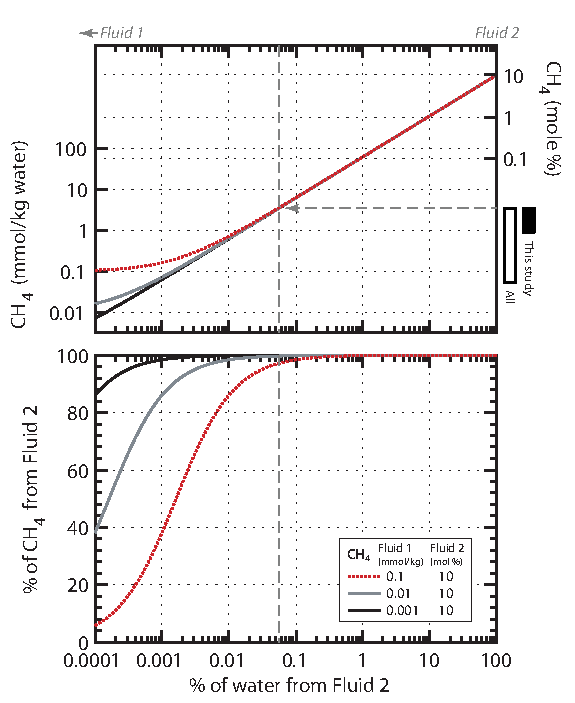
\includegraphics[width=0.65\linewidth]{figures/Fig3.6}
	\caption[Concentration of CH\textsubscript{4} in hydrothermal fluids upon mixing of a CH\textsubscript{4}-rich crustal fluid with a circulating, CH\textsubscript{4}-poor fluid]{%
		Composition
		of fluids formed by mixing of a CH\textsubscript{4}-poor
		actively-circulating seawater-derived hydrothermal fluid
		(\emph{Fluid~1}) with a CH\textsubscript{4}-rich fluid such as those
		observed in inclusions in plutonic rocks on the Southwest Indian Ridge
		and on the Mid-Atlantic Ridge (\emph{Fluid~2}) \parencite{Kelley_1996_JGR,Kelley_1997,Kelley+FruhGreen_1999_JGR}. Mixing curves are plotted for
		CH\textsubscript{4} concentrations in the \emph{Fluid~1} endmember
		ranging from 1 to 100~µmol/kg. Calculations assume that molalities of
		species other than CH\textsubscript{4} have a negligible effect on mole
		fractions in the high-CH\textsubscript{4} fluid. The black and white
		bars show CH\textsubscript{4} concentrations in vent fluids from this
		study (\autoref{tab:3:2}) and from mid-ocean ridge hydrothermal systems globally
		\parencite{Keir_2010_GRL}.
	}
	\label{fig:3:6}
\end{SCfigure*}









\textcite{Proskurowski++_2008_S} invoked abiotic reduction of aqueous
$\big\sum\!$CO\textsubscript{2} to explain the presence of high
(\textasciitilde{}1~mmol/kg) concentrations of CH\textsubscript{4} and
minor quantities (\textasciitilde{}1~µmol/kg or lower) of
C\textsubscript{2+} alkanes in vent fluids from the Lost City
hydrothermal field. They postulated a scenario that involves leaching of
primordial inorganic carbon from mantle host rocks, and subsequent
reduction of $\big\sum\!$CO\textsubscript{2} to CH\textsubscript{4} and
C\textsubscript{2+} in circulating fluids at relatively low temperature \parencite[\textless{}150~°C;][]{Proskurowski++_2006_CG}. However, Lost City
fluids contain vanishingly small amounts of $\big\sum\!$CO\textsubscript{2} because
the highly alkaline pH and high concentrations of Ca\textsuperscript{2+}
favor precipitation of carbonates, a process that proceeds rapidly at
temperatures experienced by the circulating fluids \parencite{Kelemen++_2011_AREarth,Grozeva++_2017_GCA}. The production of methane via
CO\textsubscript{2} reduction in an aqueous fluid depleted of
$\big\sum\!$CO\textsubscript{2} is therefore problematic in that it requires the addition of
mantle-derived CO\textsubscript{2} that is quickly reduced to form
CH\textsubscript{4} \parencite[up to 56\% conversion based on magmatic C/\textsuperscript{3}He ratios;][]{Proskurowski++_2008_S}, and the
remainder of which is then subsequently scavenged (presumably by
carbonate precipitation), leaving no evidence of its addition. Rates of
$\big\sum\!$CO\textsubscript{2} reduction must be comparable to or faster than
carbonate precipitation in order for CH\textsubscript{4} synthesis to
proceed in alkaline, $\big\sum\!$CO\textsubscript{2}-poor fluids such as those at
Lost City. Carbonate precipitation occurs rapidly during alteration of
peridotite \parencite{Grozeva++_2017_GCA}. In contrast, laboratory studies
consistently find sluggish reaction kinetics for the reduction of
$\big\sum\!$CO\textsubscript{2} to CH\textsubscript{4} in the presence and absence
of powdered peridotite or mafic mineral phases \parencite{McCollom+Seewald_2001_GCA,McCollom+Seewald_2003_GCA_formate,Seewald++_2006_GCA,Reeves_2010_thesis,McCollom_2016_PNAS,Grozeva++_2017_GCA}. Certain transition metal
catalysts can enhance rates of CH\textsubscript{4} production \parencite{Horita+Berndt_1999_S,Foustoukos+Seyfried_2004_S}, but H\textsubscript{2}
concentrations several orders of magnitude higher than those found in
vent fluids are required to render native Fe-Ni alloys stable \parencite{Frost_1985_JPet,Charlou++_2002_CG,Sleep++_2004_PNAS,McCollom+Bach_2009_GCA}. Furthermore, rates of CH\textsubscript{4} synthesis in fluids
deprived of $\big\sum\!$CO\textsubscript{2} are poorly-constrained, but generally
too low to be reliably detected on timescales of laboratory experiments \parencite{Fu++_2007_GCA,McCollom_2012_PNAS_comment,McCollom_2013_RiMG}.

Data from other vent fields are also inconsistent with synthesis of
CH\textsubscript{4} on timescales associated with actively-circulating
fluids. At the basalt-hosted Lucky Strike field, synthesis of methane
within the low-H\textsubscript{2} fluids discharging at the Medea and
Isabel vents is thermodynamically disfavored at \emph{in situ}
temperatures (270--292~°C; \autoref{tab:3:2} and \mrefs[D]{Fig.}{fig:3:3}). With increasing
temperature, methane formation becomes even more unfavorable (\mrefs[A]{Fig.}{fig:3:2}),
and thus aqueous CO\textsubscript{2} reduction at the higher
temperatures (possibly as high as 475~°C) the fluids have experienced
here \parencite{Pester++_2012_GCA} is also unsupported. Concentrations of
CH\textsubscript{4} shows no relation to either $\big\sum\!$CO\textsubscript{2} or
H\textsubscript{2} in the Lucky Strike fluids here \parencite[see discussion and Fig.~2 in][]{Pester++_2012_GCA}. These data indicate that
CH\textsubscript{4} did not form from reduction of $\big\sum\!$CO\textsubscript{2}
during migration of magmatic CO\textsubscript{2} between degassing from
the magma chamber at \textasciitilde{}3000~mbsf (meters below seafloor)
and venting at the seafloor. Taken together, this evidence suggests that
CH\textsubscript{4} originates not within an actively-convecting
hydrothermal fluid, but is produced elsewhere and entrained into the
circulating fluid.

The magmatic volatiles from which CH\textsubscript{4} forms may be
sourced from gabbroic rocks formed from cooling of volatile-bearing
melts beneath mid-ocean ridges. Oxidized carbon (as CO\textsubscript{2})
is generally considered to exhibit near-perfect incompatibility, such
that during decompression melting, nearly all carbon originally in the
suboceanic mantle partitions into the melt fraction, leaving very little
behind in residual peridotite. Estimates of the amount of carbon in the
mantle suffer from large uncertainties, but are typically in the range
of 20 to 300~ppm carbon \parencite{Dasgupta+Hirschmann_2010_EPSL}. Serpentinitized
oceanic peridotites from several mid-ocean ridges contain up to 1500~ppm
carbon, and are therefore a sink for carbon \parencite{Alt++_2013_L}. Carbon
in these rocks is thought to exist mostly as condensed phases \parencite{FruhGreen++_2004}, consistent with more recent observational and
theoretical considerations \parencite{Menez++_2012_NG,Pasini++_2013_L,Milesi++_2016_GCA}. In contrast, gabbros from the same areas contain
less carbon (up to 300~ppm), primarily hosted in inclusions bearing
CO\textsubscript{2}, CH\textsubscript{4} and/or graphite \parencite{FruhGreen++_1996_ODP-SR,Kelley+FruhGreen_1999_JGR,Kelley+FruhGreen_2001_GCA}.
These petrological constraints suggest that magmatic volatiles entrapped
in gabbros, but probably not fresh peridotites, are a potential source
for carbon in CH\textsubscript{4} at oceanic spreading centers.
Additionally, migration of magmatic volatiles out of melts directly into
layers of gabbro or peridotite may also enable carbon to come in contact
with reducing conditions conducive to methane synthesis.

The occurrence and composition of methane-rich aqueous fluids within the
sub-oceanic ridge lithosphere is recorded by secondary fluid inclusions
hosted in plutonic rocks. \textcite{Kelley_1996_JGR,Kelley_1997,Kelley+FruhGreen_1999_JGR} documented several types of abundant volatile-rich inclusions in
gabbros recovered from the slow-spreading Southwest Indian and
Mid-Atlantic Ridges by several Ocean Drilling Program (ODP) expeditions.
A common type of inclusion occurring along healed microcracks in
plagioclase grains contained up to 47\% CH\textsubscript{4} (with
balance of H\textsubscript{2}O). Temperatures indicated by
CO\textsubscript{2}--CH\textsubscript{4} carbon isotope geothermometry
(300--600~°C) and homogenization temperatures of the Southwest Indian
Ridge fluid inclusions (350--370~°C, corresponding to entrapment at
\emph{in situ} temperatures of ca.\ 400~°C) \parencite{Kelley+FruhGreen_1999_JGR}
agree with clumped isotopologue temperatures, and are compatible with
formation of CH\textsubscript{4} during re-speciation of occluded
magmatic volatiles as the host gabbros cooled to below 400~°C (\mrefs[A]{Fig.}{fig:3:2}).
While δ\textsuperscript{13}C values of CH\textsubscript{4} measured in
fluid inclusions are somewhat lower \parencite[$-$34 to $-$20‰;][]{Kelley+FruhGreen_1999_JGR} than observed values in vent fluids ($-$18 to $-$9‰; \autoref{tab:3:S1}), carbon isotopic data for inclusions may be affected by
potential background sources either endogenous to the crushed mineral
separates, introduced during sample handling, or formed during the
stepped heating experiments. These background sources of carbon typically
have relatively low δ\textsuperscript{13}C values of $-$25 to $-$30‰ \parencite{DesMarais_1986_EPSL,Miller+Pillinger_1997_GCA}.

Graphite is stable under conditions characterizing many hydrothermal
settings \parencite{Luque++_2009_G,Rumble_2014_E}. At isotopic equilibrium,
graphite is \textasciitilde{}10‰ enriched in \textsuperscript{13}C relative to
CH\textsubscript{4} at temperatures of 300 to 400~°C \parencite{Bottinga_1969_GCA}.
It is worth noting that in all mid-ocean ridge hydrothermal fluids,
δ\textsuperscript{13}C values of CH\textsubscript{4} are lower than
mantle-derived CO\textsubscript{2} ($-$5‰, \mrefs[A]{Fig.}{fig:3:1}). Relatively uniform
δ\textsuperscript{13}C values ($-$19‰ to $-$9‰) are observed in vent fluids
with high (millimolar) CH\textsubscript{4} contents \parencite{McCollom+Seewald_2007_CR,Keir_2010_GRL}. Furthermore,
CH\textsubscript{4}/\textsuperscript{3}He ratios in vent fluids \parencite[see][]{Keir_2010_GRL} indicate less-than-quantitative conversion
(\textasciitilde{}0.2\% to 50\%) of mantle carbon to CH\textsubscript{4}
 \parencite[C/\textsuperscript{3}He \textasciitilde{} 1×10\textsuperscript{9},][]{Marty+Tolstikhin_1998_CG}. Precipitation of graphite from a
CH\textsubscript{4}-rich fluid entrapped in plutonic rocks may explain
both the missing carbon \parencite{McDermott++_2015_PNAS} and the observed
δ\textsuperscript{13}C values \parencite{Luque++_2012_GFront}.

\autoref{fig:3:S1} shows predictions from a thermodynamic model of an
ideal graphite-saturated C--O--H vapor with oxygen fugacity given by the
fayalite-magnetite-quartz (FMQ) mineral buffer assemblage and a total
pressure of 1~kbar. Calculations show that precipitation of graphite
concomitant with methane formation is favored at ca.\ 400~°C and under
water-poor conditions, consistent with many previous investigations \parencite{French_1966_RG,Eugster+Skippen_1967,Ohmoto+Kerrick_1977_AJS,Holloway_1984_G,FruhGreen++_2004}. Predicted
C\textsubscript{1}/C\textsubscript{2} ratios are also consistent with
measured values in vent fluids \parencite[][and \autoref{fig:3:S1}]{McDermott_2015_thesis}.
Propane (C\textsubscript{3}) is in excess by two orders of magnitude
compared with thermodynamic equilibrium at \textasciitilde{}300~°C
\parencite[][and \autoref{fig:3:S1}]{McDermott_2015_thesis}. To explain the relative
proportions of ethane and propane (and butanes) at this temperature
requires both a high CH\textsubscript{4} fugacity and (paradoxically) a
low H\textsubscript{2} fugacity of several log units below (more
oxidized than) FMQ. Generation of small amounts of C\textsubscript{2+}
hydrocarbons (\textasciitilde{}1~µM or less) from the thermal breakdown
of dissolved organic matter carried in recharging seawater
(\textasciitilde{}40~µM) may account for the excess propane and butanes
relative to ethane and methane. Alternatively, the C\textsubscript{2+}
hydrocarbons may not have equilibrated at a uniform temperature
\parencite{McDermott_2015_thesis}, or may be formed via low-yield, kinetically-throttled
reactions occurring in circulating fluids \parencite{Foustoukos+Seyfried_2004_S}. Regardless of their specific origins, similarities in the
abundances and isotopic compositions of low molecular weight
hydrocarbons in vent fluids at Von Damm and other hot-spring systems at
slow-spreading ridges suggest that they may share common origins.

Concentrations of CH\textsubscript{4} in the gabbro-hosted inclusions
from the Southwest Indian Ridge and from other slow-spreading areas can
be several orders of magnitude greater than those observed in
corresponding vent fluids \parencite{Kelley_1996_JGR,Kelley_1997}. Mass-balance
considerations suggest that extraction of CH\textsubscript{4}-rich
fluids occluded in gabbros can explain CH\textsubscript{4}
concentrations at all known sediment-free mid-ocean ridge hydrothermal
fields. Mixing curves plotted in \autoref{fig:3:6} show that addition of less than
0.1\% of a CH\textsubscript{4}--H\textsubscript{2}O fluid of similar
composition to those indicated by the inclusions (\emph{Fluid 2} in the
figure) to a CH\textsubscript{4}-poor circulating hydrothermal fluid
(\emph{Fluid 1}) is sufficient to match even the highest
CH\textsubscript{4} concentrations seen in vent fluids. Assuming carbon
contents ranging from 30 to 300~ppm in the gabbro \parencite{Kelley+FruhGreen_1999_JGR}, water-to-rock ratios between 0.8 and 8 are required
to explain CH\textsubscript{4} concentrations of up to 3~mmol/kg in vent
fluids assuming all carbon in gabbro existed as leachable
CH\textsubscript{4}. Lower water-to-rock ratios are necessary if
conversion efficiency is less than 100\% (e.g., due to graphite
precipitation) or if lower initial carbon contents are assumed.
Constraints from mobile inorganic elements (e.g., Li, Rb, Sr) generally
indicate that water/rock ratios are substantially lower than
\textasciitilde{}10 in many mid-ocean ridge hydrothermal systems \parencite{VonDamm++_1985_GCA_EPR,Berndt++_1989_GCA} with values of 0.4 to 6
calculated for the subsurface at Von Damm \parencite{McDermott_2015_thesis} and 2 to 4
at Lost City  \parencite{Foustoukos++_2008_GCA} for example.


While only slow-spreading environments were investigated in this study,
we hypothesize that the same origin of methane applies at sites on the
fast-spreading East Pacific Rise, particularly given the similar
δ\textsuperscript{13}C values of methane there \parencite{Welhan+Craig_1983}.
The fact that these hydrothermal fluids contain low C\textsubscript{2+}
along with low CH\textsubscript{4} concentrations \parencite{Keir_2010_GRL,Welhan_1988_CG} suggests a genetic link between CH\textsubscript{4} and the
C\textsubscript{2+} hydrocarbons. Differences in axial structure and
tectonism may account for the difference in hydrocarbon content of vent
fluids at fast- and slow-spreading ridges. At magma-poor slow-spreading
ridges, extension is accommodated primarily by detachment faulting, as
opposed to magmatic emplacement of new crust that characterizes
fast-spreading ridges \parencite{Buck++_2005_N,Dunn_2007_TiG}. Low-angle,
large-offset, and long-lived (\textgreater{}1 Myr) normal faults near
vent fields at slow-spreading ridges allow for fluid penetration deep
into plutonic rocks of layer 3, enabling access to fresh gabbroic
material and/or inclusions to be leached \parencite{Kelley_1996_JGR,Schroeder++_2002_G,Schlindwein+Schmid_2016_N}. In contrast, in fast spreading
environments such as the East Pacific Rise, shallow melt lenses at 1 to
2~km below seafloor may limit the depth of circulation \parencites(e.g.,)()[][]{Hasenclever++_2014_N}[and references in][]{Alt_1995_AGU-GM}.

\section{Conclusions}\label{conclusions}

Methane clumped isotopologue data obtained for fluids venting from
diverse unsedimented mid-ocean ridge hydrothermal systems uniformly
indicate temperatures of last equilibration of ca.\ 300~°C. Taken in
combination with geochemical and geologic observations and reaction
rates determined in experiments, the
Δ\textsuperscript{13}CH\textsubscript{3}D data provide evidence that
abiotic reduction of $\big\sum\!$CO\textsubscript{2} at
low temperatures (\textless{}200~°C) is not a significant source of
methane over timescales characterizing convective hydrothermal
circulation at oceanic spreading centers. Furthermore, consideration of
volatile contents and C--O--H speciation in melt-derived plutonic rocks
and residual peridotites suggests that temperature, pressure,
\(f_{\mathrm{O}_{\mathrm{2}}}\), and
\(f_{\mathrm{H}_{\mathrm{2}}\mathrm{O}}\) conditions conducive to
methane synthesis may be widespread in the oceanic crust.

Two hypotheses were considered for explaining the origin of
CH\textsubscript{4} in hydrothermal fluids: (\emph{i}) aqueous synthesis
of CH\textsubscript{4} during active circulation and (\emph{ii})
extraction of CH\textsubscript{4}-rich fluids occluded in plutonic
rocks. While both are conceivably compatible with the methane
isotopologue data when taken in isolation, clumped isotopologue
temperatures indicate that formation of CH\textsubscript{4} from
$\big\sum\!$CO\textsubscript{2} at Lost City does not occur at temperatures
\textless{}200~°C in the upflow. Furthermore, the former scenario is not
compatible with thermodynamic, radioisotopic, and mass balance
constraints at several sites. These lines of evidence lead us to favor
the latter hypothesis, which invokes a more straightforward scenario
wherein vent fluids with millimolar quantities of CH\textsubscript{4}
represent mixtures of a minute amount of a CH\textsubscript{4}-rich
fluid (of hypogene origin) with a large volume of an
actively-circulating, CH\textsubscript{4}-poor fluid. Proportions of
mixing may be determined by the relative access that circulating fluids
have to magmatic volatile-bearing rocks of the plutonic foundation. This
could also explain apparent relationships of CH\textsubscript{4}
concentration in vent fluids to tectonic setting and host rock
lithology. Efforts to distinguish between the CH\textsubscript{4}
contributed via these pathways will benefit from rigorous interrogation
of factors governing fluid flow and chemical kinetics in
hydrothermally-influenced settings.

The new data also provide constraints on the closure temperature of
hydrogen exchange between methane and water. The observation of sluggish
or indiscernible exchange of H among methane isotopologues below ca.
270~°C on timescales of \textasciitilde{}10\textsuperscript{2}~years is
relevant not only to the application of clumped isotope measurements as
a novel geothermometer, but also provides information about the
stability of the C--H bond in hydrocarbons in nature. Given the
increasing appreciation of hydrocarbon-water-mineral interactions in
economically important settings \parencite{Seewald_2003_N}, insights of this nature
may find utility in studies of the origin and composition of aqueous and
organic fluids in the Earth's subsurface.

\section*{Acknowledgments}\label{acknowledgments-1}

We thank Frieder Klein, Wolfgang Bach, and Grant Garven for helpful
discussions regarding the petrology and plumbing of hydrothermal
systems. Grants from the National Science Foundation (NSF EAR-1250394 to
S.O.), NASA Astrobiology Institute (NAI \#024461), N. R. Braunsdorf and D. J. H.
Smit of Shell PTI/EG and the Deep Carbon Observatory (to S.O.) supported
this work. S.O. thanks the Kerr-McGee Professorship at MIT. This
research was conducted with Government support under and awarded by U.S.
Department of Defense, Office of Naval Research, National Defense
Science and Engineering Graduate (NDSEG) Fellowship (to D.T.W.), 32 CFR
168a. D.T.W. was also supported via a Shell-MITEI fellowship.


\begin{figure*}
	\centering
	\includegraphics[width=0.95\linewidth]{figures/Fig3.S1}
	\caption[Equilibrium composition of a graphite-saturated C--O--H fluid at 1000~bar with \(f_{\mathrm{O}_{\mathrm{2}}}\) = FMQ]{Equilibrium composition of a
		graphite-saturated C--O--H fluid at 1000~bar (\textbf{A}) with oxygen
		fugacity (\(f_{\mathrm{O}_{\mathrm{2}}}\)) given by the
		fayalite-magnetite-quartz (FMQ) redox buffer (\textbf{B}). The modeled
		fluid is an ideal gas consisting of CO, CO\textsubscript{2},
		H\textsubscript{2}, H\textsubscript{2}O, O\textsubscript{2}, ethane, and
		propane. The model is essentially that of \textcite{French_1966_RG}, with the addition of C\textsubscript{2+} compounds (as also considered by \textcite{Kawagucci++_2013_CG,McDermott_2015_thesis}, with different assumptions regarding redox, water activity, and total mass of carbon). To calculate the
		composition of the fluid, equilibrium constants were computed at various
		temperatures using CHNOSZ \parencite{Dick_2008_GT} from tabulated standard molal
		thermodynamic properties and equation of state parameters \parencite{CHNOSZ_Kel60,CHNOSZ_HDN+78,CHNOSZ_HOK+98,CHNOSZ_WEP+82,Johnson++_1992_CnG,CHNOSZ_Sho93}, the fugacities of CO and CO\textsubscript{2} were
		calculated, and then the fugacities of all other gaseous species were
		solved iteratively under the constraint that $\big\sum\!$\emph{f} = 1000~bar \parencite[a
		pressure typical of those indicated by fluid inclusion studies;][]{Vanko_1988_JGR}. Graphite is unstable above \textasciitilde{}500~°C, as shown
		by the equilibrium fugacities of CO+CO\textsubscript{2} exceeding the
		pressure of the system (dashed lines in A). Ratios of fugacities of
		selected species show that CH\textsubscript{4} is the dominant gas-phase
		species below \textasciitilde{}400~°C (\textbf{C}), and that predicted
		ratios of C\textsubscript{1}/C\textsubscript{2} and
		C\textsubscript{2}/C\textsubscript{3} are
		\textasciitilde{}10\textsuperscript{3} to 10\textsuperscript{4} between
		200 and 400~°C (\textbf{D}, \textbf{E}). Dotted lines in (D) and (E)
		mark the range of C\textsubscript{1}/C\textsubscript{2} and
		C\textsubscript{2}/C\textsubscript{3} measured in hydrothermal fluids
		from the four vent fields we studied \parencite{Charlou++_2000_CG,Charlou++_2002_CG,Proskurowski++_2008_S,McDermott++_2015_PNAS}. The vapor pressure
		curve of water at 1000~bar is shown in blue in (A). Values of
		\(\log f_{\mathrm{H}_{\mathrm{2}}\mathrm{O}}\) that plot above this
		curve are inaccessible because the presence of liquid water sets the
		fugacity of H\textsubscript{2}O and causes the fugacities of
		O\textsubscript{2} and all other species to adjust accordingly.
		Therefore, values of
		\(\log\left({f_{\mathrm{C}\mathrm{H}_{\mathrm{4}}}}\middle/{f_{\mathrm{H}_{\mathrm{2}}\mathrm{O}}}\right) > 0\)
		do not necessarily indicate that total CH\textsubscript{4} content
		exceeds total water content when multiple fluid phases coexist. Liquid
		water has been neglected in our model, but calculations in which
		H\textsubscript{2}O(\emph{l}) is explicitly considered show that
		graphite, an H\textsubscript{2}O-dominated liquid, and a
		CH\textsubscript{4}-rich gas phase can coexist at
		\textasciitilde{}400~°C and \(f_{\mathrm{O}_{\mathrm{2}}}\) close to FMQ
		\parencite{Holloway_1984_G}.}
	\label{fig:3:S1}
\end{figure*}





\begin{figure*}
	\centering
	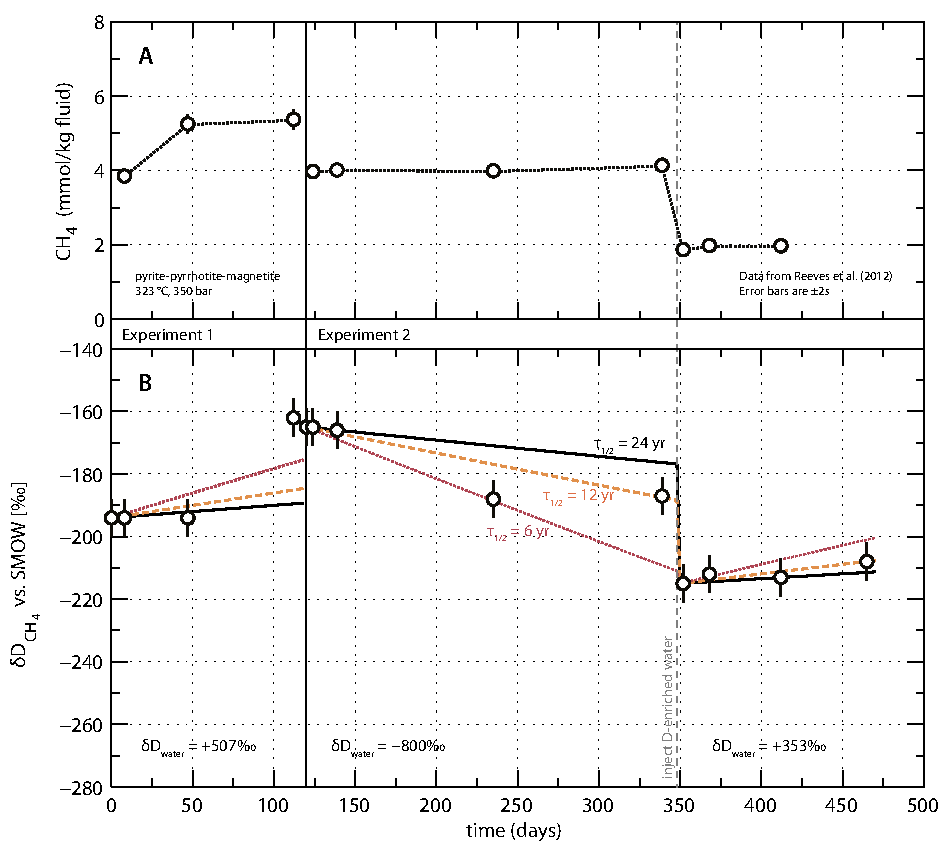
\includegraphics[width=0.95\linewidth]{figures/Fig3.S2}
	\caption[Rates of hydrogen exchange between CH\textsubscript{4}(\emph{aq}) and
	H\textsubscript{2}O(\emph{l}) from data of \textcite{Reeves++_2012_GCA} ]{%
		Experimental constraints on hydrogen
		exchange between CH\textsubscript{4}(\emph{aq}) and
		H\textsubscript{2}O(\emph{l}) from two experiments conducted by \textcite{Reeves++_2012_GCA} in a flexible cell hydrothermal apparatus at 323~°C and
		350~bar. Concentrations of CH\textsubscript{4} (\textbf{A}) remain
		indistinguishable within analytical error (±5\%, 2\emph{s}) in
		Experiment~2, but not in Experiment~1, perhaps due to calibration or operator error as noted by those authors. Measured
		pH was \textasciitilde{}4.2, and concentrations of H\textsubscript{2}
		and $\big\sum\!$H\textsubscript{2}S were 0.26--0.7 mmol/kg fluid and
		\textasciitilde{}11~mmol/kg fluid, respectively, consistent with
		predictions for a Fe--S--O--H fluid buffered by PPM at experimental
		conditions \parencite{Reeves++_2012_GCA}. Panel (\textbf{B}) shows measurements
		of D/H of CH\textsubscript{4} compared against modeled kinetics for D/H
		exchange with varying half-exchange time ($\tau_{1/2} = \ln(2)/k$). The modeled kinetics assume that CH\textsubscript{4}
		concentration is constant, the rate of isotopic exchange is first order
		in CH\textsubscript{4}, and the equilibrium D/H fractionation factor
		{[}$\varepsilon = $ (D/H)\textsubscript{methane}/(D/H)\textsubscript{water} -- 1{]} is
		$-$130‰ (see \autoref{fig:3:5}). We take $\tau_{1/2}$ = 24~yr (black curve)
		as a best-guess estimate of the rate of true isotopic exchange; this
		value is shown in \autoref{fig:3:4}.
	}
	\label{fig:3:S2}
\end{figure*}






\begin{landscape}	
	
	\centering
	
	\begin{ThreePartTable}	
			
		\begin{TableNotes}
			\item Abbreviations: mm, mmol/kg fluid; mM, mmol/L fluid.
			
			\item Data sources: (1) this study; (2) \textcite{Reeves++_2014_PNAS}; (3) \textcite{Charlou++_2010}; (4) \textcite{Proskurowski++_2006_CG}; (5) \textcite{Welhan+Craig_1983};
			(6) \textcite{Horibe+Craig_1995_GCA}; (7) \textcite{Kawagucci++_2010_JGR}; (8) \textcite{Kumagai++_2008_Gf}; (9) \textcite{McDermott++_2015_PNAS}.
			
			\item Notes: † cf. \emph{T}\textsubscript{max} 96~°C in ref.~2; ‡ phase-separated; § snail colony; ¶ shrimp colony
			
			\item \textsuperscript{a} Dash (---) indicates that data were not reported or
			that samples were unable to be matched across multiple references.
			
			\item \textsuperscript{b} Maximum measured vent temperature.
			
			\item \textsuperscript{c} Asterisk (*) indicates near-endmember fluid sample
			(represented by stars in \autoref{fig:3:5}). For these samples, concentrations of
			$\big\sum\!$CO\textsubscript{2}, H\textsubscript{2}, and CH\textsubscript{4} and
			δ\textsuperscript{13}C values of $\big\sum\!$CO\textsubscript{2} have been
			extrapolated to endmember fluid composition (regressed to zero Mg
			content) assuming entrainment of seawater containing \textasciitilde{}53~mM Mg.
			
			\item \textsuperscript{d} Endmember vent fluids typically have δD values of
			H\textsubscript{2}O between $-$2 and +4‰ \parencite{Shanks++_1995_AGU-GM}. A value of
			0‰ was assumed when no data could be found (see text and \autoref{fig:3:5}).
			
			\item \textsuperscript{e} Values are as reported; it is not known whether
			correction for $\big\sum\!$CO\textsubscript{2} in seawater was applied.
			
		\end{TableNotes}
		
		\setlength{\tabcolsep}{10pt}
		\setlength{\abovetopsep}{9pt}
		\small
		
		\begin{longtable}[]{@{} ll d{0}l lll ll @{\hskip 0.2em} p{0.01em} lll l @{}}
			
			\tabularnewline  % adds padding!
			\tabularnewline
			\caption[Compilation of δD values of \ce{CH4} \& \ce{H2} and associated data]{Compilation of hydrogen isotope ratios of CH\textsubscript{4} and
				H\textsubscript{2} and associated data on vent fluids from sediment-poor
				hydrothermal systems.}\label{tab:3:S1}\\ 	% this \\ is very important !!
			\toprule
			\multirow{2}{*}{Field} & \multirow{2}{*}{Vent}  & \multirow{2}{*}{\shortstack[l]{\emph{T}\textsubscript{max}\\ (°C)\textsuperscript{b}}}  & \multirow{2}{*}{\shortstack[l]{Mg\\ (mM)}}  & \multirow{2}{*}{\shortstack[l]{$\big\sum\!$\ce{CO2}\\ (mm)}}  & \multirow{2}{*}{\shortstack[l]{\ce{H2}\\ (mM)}}  & \multirow{2}{*}{\shortstack[l]{\ce{CH4}\\ (mM)}} & \multicolumn{2}{c}{δ\textsuperscript{13}C (‰)} & & \multicolumn{3}{c}{δD (‰)} & \multirow{2}{*}{Notes}\tabularnewline
			\cmidrule{8-9} \cmidrule{11-13}
			 &  &  &   &   &   &   & $\big\sum\!$CO\textsubscript{2} & CH\textsubscript{4} & &
			CH\textsubscript{4} & H\textsubscript{2} &
			H\textsubscript{2}O\textsuperscript{d} &\tabularnewline
			\midrule
			\endfirsthead
%
			\tabularnewline
			\tabularnewline			
			\caption[]{Compilation of hydrogen isotope ratios of CH\textsubscript{4} and
				H\textsubscript{2} and associated data (\textit{continued}).}\\ 	% this \\ is very important !!
			\toprule
			\multirow{2}{*}{Field} & \multirow{2}{*}{Vent}  & \multirow{2}{*}{\shortstack[l]{\emph{T}\textsubscript{max}\\ (°C)\textsuperscript{b}}}  & \multirow{2}{*}{\shortstack[l]{Mg\\ (mM)}}  & \multirow{2}{*}{\shortstack[l]{$\big\sum\!$\ce{CO2}\\ (mm)}}  & \multirow{2}{*}{\shortstack[l]{\ce{H2}\\ (mM)}}  & \multirow{2}{*}{\shortstack[l]{\ce{CH4}\\ (mM)}} & \multicolumn{2}{c}{δ\textsuperscript{13}C (‰)} & & \multicolumn{3}{c}{δD (‰)} & \multirow{2}{*}{Notes}\tabularnewline
			\cmidrule{8-9} \cmidrule{11-13}
			 &  &  &   &   &   &   & $\big\sum\!$CO\textsubscript{2} & CH\textsubscript{4} & &
			CH\textsubscript{4} & H\textsubscript{2} &
			H\textsubscript{2}O\textsuperscript{d} &\tabularnewline
			\midrule
			\endhead
			
			\midrule
			\multicolumn{14}{r}{\textit{Continued on next page}}
			\tabularnewline
			\tabularnewline
			\endfoot
%			\begin{minipage}[b]{0.07\columnwidth}\raggedright\strut
%				Field\strut
%			\end{minipage} & \begin{minipage}[b]{0.07\columnwidth}\raggedright\strut
%				Vent\textsuperscript{a}\strut
%			\end{minipage} & \begin{minipage}[b]{0.07\columnwidth}\raggedright\strut
%				\emph{T}\textsubscript{max}
%				
%				(°C)\textsuperscript{b}\strut
%			\end{minipage} & \begin{minipage}[b]{0.07\columnwidth}\raggedright\strut
%				Mg
%				
%				(mM)\textsuperscript{c}\strut
%			\end{minipage} & \begin{minipage}[b]{0.07\columnwidth}\raggedright\strut
%				$\big\sum\!$CO\textsubscript{2}
%				
%				(mm)\strut
%			\end{minipage} & \begin{minipage}[b]{0.07\columnwidth}\raggedright\strut
%				H\textsubscript{2}
%				
%				(mM)\strut
%			\end{minipage} & \begin{minipage}[b]{0.07\columnwidth}\raggedright\strut
%				CH\textsubscript{4}
%				
%				(mM)\strut
%			\end{minipage} & \begin{minipage}[b]{0.07\columnwidth}\raggedright\strut
%				δ\textsuperscript{13}C (‰)\strut
%			\end{minipage} & \begin{minipage}[b]{0.07\columnwidth}\raggedright\strut
%				\strut
%			\end{minipage} & \begin{minipage}[b]{0.07\columnwidth}\raggedright\strut
%				δD (‰)\strut
%			\end{minipage} & \begin{minipage}[b]{0.07\columnwidth}\raggedright\strut
%				Notes\strut
%			\end{minipage}\tabularnewline
%			
%			& & & & & & & $\big\sum\!$CO\textsubscript{2} & CH\textsubscript{4} & &
%			CH\textsubscript{4} & H\textsubscript{2} &
%			H\textsubscript{2}O\textsuperscript{d} &\tabularnewline
%			& & & & & & & & & & & & &\tabularnewline
			
			\insertTableNotes\\
			\endlastfoot
			
			&\tabularnewline
			\multicolumn{5}{@{}l}{\textit{Mid-Atlantic Ridge}}  & & & &\tabularnewline
			Rainbow & Guillaume (X4) & 361 & 0* & 24.3 & 16.5 & 2.13 & --- & $-$17.6 &
			& $-$98 & --- & --- & (1, 2)\tabularnewline
			& CMSP\&P & 365 & 0* & 21.9 & 15.9 & 2.05 & --- & $-$17.5 & & $-$98 & --- &
			--- & (1, 2)\tabularnewline
			& Auberge (X3) & 370 & 0* & 22.8 & 15.7 & 2.16 & --- & $-$17.4 & & $-$98 &
			--- & --- & (1, 2)\tabularnewline
			& --- & 365 & 0* & 16 & 16 & 2.5 & $-$3.2\textsuperscript{e} & $-$17.7 & &
			$-$105 & $-$356 & --- & (3)\tabularnewline
			& --- & 360 & 0* & 17 & 13 & 1.6 & $-$2.5\textsuperscript{e} & $-$17.8 & &
			$-$107 & $-$379 & --- & (3)\tabularnewline
			Lost City & Beehive & 94 & 0* & 0.18 & 10.4 & 1.08 & --- & $-$10.9 & &
			$-$127 & --- & --- & (1, 2)\tabularnewline
			& & 90 & 0* & --- & --- & --- & --- & --- & & $-$127 & $-$609 & +2 to 7 &
			(4)\tabularnewline
			& & 90 & 0* & --- & --- & --- & --- & --- & & $-$126 & $-$609 & +2 to 7 &
			(4)\tabularnewline
			& Marker 6 & 67 & 0* & --- & --- & --- & --- & --- & & $-$108 & $-$605 & +2
			to 7 & (4) {†}\tabularnewline
			& & 62 & 0* & --- & --- & --- & --- & --- & & $-$129 & $-$616 & +2 to 7 &
			(4) {†}\tabularnewline
			& IMAX (IF) & 55 & --- & --- & --- & --- & --- & --- & & $-$129 & $-$649 &
			+2 to 7 & (4)\tabularnewline
			& & 55 & --- & --- & --- & --- & --- & --- & & $-$139 & $-$646 & +2 to 7 &
			(4)\tabularnewline
			& & 55 & --- & --- & --- & --- & --- & --- & & $-$136 & $-$648 & +2 to 7 &
			(4)\tabularnewline
			& Marker 7 & 28 & --- & --- & --- & --- & --- & --- & & $-$129 & $-$663 & +2
			to 7 & (4)\tabularnewline
			& & 28 & --- & --- & --- & --- & --- & --- & & $-$125 & $-$666 & +2 to 7 &
			(4)\tabularnewline
			& Marker 8 & 43 & --- & --- & --- & --- & --- & --- & & $-$141 & $-$658 & +2
			to 7 & (4)\tabularnewline
			& & 43 & --- & --- & --- & --- & --- & --- & & $-$136 & $-$651 & +2 to 7 &
			(4)\tabularnewline
			& Marker C & 62 & --- & --- & --- & --- & --- & --- & & $-$126 & $-$620 & +2
			to 7 & (4)\tabularnewline
			& & 70 & --- & --- & --- & --- & --- & --- & & $-$130 & $-$614 & +2 to 7 &
			(4)\tabularnewline
			& Marker H & 60 & --- & --- & --- & --- & --- & --- & & $-$99 & $-$657 & +2
			to 7 & (4)\tabularnewline
			& & 60 & --- & --- & --- & --- & --- & --- & & $-$104 & $-$689 & +2 to 7 &
			(4)\tabularnewline
			& Marker 3 & 61 & --- & --- & --- & --- & --- & --- & & $-$112 & $-$610 & +2
			to 7 & (4)\tabularnewline
			& & 71 & --- & --- & --- & --- & --- & --- & & $-$103 & $-$605 & +2 to 7 &
			(4)\tabularnewline
			& & 73 & --- & --- & --- & --- & --- & --- & & $-$125 & $-$609 & +2 to 7 &
			(4)\tabularnewline
			& --- & 93 & 0* & --- & --- & --- & --- & $-$11.9 & & $-$130 & $-$618 & --- &
			(3)\tabularnewline
			
%			&\tabularnewline
			Broken Spur & --- & 353 & 0* & --- & --- & --- & --- & --- & & --- &
			$-$393 & --- & (4)\tabularnewline
			\tabularnewline
			Logatchev (1?) & --- & 350 & 0* & --- & --- & --- & --- & --- & & $-$109 & $-$372
			& --- & (4)\tabularnewline
			Logatchev 1 & --- & 346 & 0* & 3.6 & 9 & 2.0 & +4.1\textsuperscript{e} &
			$-$10.2 & & $-$104 & $-$350 & --- & (3)\tabularnewline
			& --- & 352 & 0* & 4.4 & 13 & 2.6 & +7.4\textsuperscript{e} & $-$10.3 & &
			$-$104 & $-$360 & --- & (3)\tabularnewline
			Logatchev 2 & --- & 320 & 0* & 6.2 & 11 & 1.2 & +9.5\textsuperscript{e}
			& $-$6.1 & & $-$93 & $-$231 & --- & (3) {‡}\tabularnewline
			Ashadze 1 & --- & 353 & 0* & 3.7 & 8 & 0.5 & +2.1\textsuperscript{e} &
			$-$12.3 & & $-$104 & $-$333 & --- & (3)\tabularnewline
			& --- & 353 & 0* & --- & 19 & 1.2 & +4.6\textsuperscript{e} & $-$14.1 & &
			$-$101 & $-$343 & --- & (3)\tabularnewline
			Ashadze 2 & --- & 296 & 0* & --- & 26 & 0.8 & +0.2\textsuperscript{e} &
			$-$8.7 & & $-$107 & $-$270 & --- & (3) {‡}\tabularnewline
			Lucky Strike & Medea & 270 & 0* & 98 & 0.063 & 0.89 & --- & $-$14.2 & &
			$-$99 & --- & --- & (1, 2)\tabularnewline
			& Isabel & 292 & 0* & 112 & 0.034 & 0.86 & --- & $-$12.6 & & $-$100 & --- &
			--- & (1, 2)\tabularnewline
			& & & & & & & & & & & & &\tabularnewline
			\multicolumn{5}{@{}l}{\textit{East Pacific Rise}} & &  & & &\tabularnewline
			9° N & --- & 380 & 0* & --- & --- & --- & --- & --- & & --- & $-$328 & ---
			& (4)\tabularnewline
			21° N & Nat. Geo. Soc. & 350 & 0* & --- & 30.5 & 1.4 & $-$7.0 & $-$15.0 & &
			$-$102 & $-$401 & +0.5 & (5, 6)\tabularnewline
			& & & & & & & & & & & & &\tabularnewline
			\multicolumn{5}{@{}l}{\textit{Central Indian Ridge}}  & & & &\tabularnewline
			Kairei & Kali & 362 & 0* & 8.0 & 3.3 & 0.12 & $-$5.3 & $-$9.8 & & --- & $-$368
			& --- & (7, 8)\tabularnewline
			& & 316 & 8.4 & 12.1 & 3.6 & --- & --- & --- & & --- & $-$328 & --- & (7,
			8)\tabularnewline
			& Monju & 299 & 5.2 & 7.9 & 2.1 & --- & --- & --- & & --- & $-$385 & --- &
			(7, 8)\tabularnewline
			& & 42 & 50.9 & 9.3 & 8×10\textsuperscript{$-$4} & --- & --- & --- & & ---
			& $-$431 & --- & (7, 8)\tabularnewline
			& & 87 & 43.7 & 6.0 & 0.69 & --- & --- & --- & & --- & $-$361 & --- & (7,
			8) {§} \tabularnewline
			& & 22 & 48.3 & 12.6 & 0.13 & --- & --- & --- & & --- & $-$493 & --- & (7,
			8) {§}\tabularnewline
			& Fugen & 305 & 4.5 & 9.5 & 2.7 & --- & --- & --- & & --- & $-$391 & --- &
			(7, 8)\tabularnewline
			& Daikoku  & 306 & 0* & --- & 2.2 & --- & --- & --- & & --- &
			$-$340 & --- & (7)\tabularnewline
			& --- & 350 & 0* & --- & --- & --- & --- & --- & & --- & $-$400 & --- &
			(4)\tabularnewline
			Edmond & Nura Nura & 375 & 0* & 12.8 & 0.11 & 0.31 & $-$5.5 & $-$13.5 & &
			--- & $-$362 & --- & (7, 8)\tabularnewline
			& Marker 27 & 325 & 0* & 12.3 & 0.10 & --- & --- & --- & & --- & $-$377 &
			--- & (7, 8)\tabularnewline
			& White Head & 263 & 12.4 & 8.1 & 0.04 & --- & --- & --- & & --- & $-$412
			& --- & (7, 8)\tabularnewline
			& Gr.\ Shrimp V.\ & 281 & 13.4 & 12.1 & 0.48 & --- & --- & --- & &
			--- & $-$681 & --- & (7, 8) {¶} \tabularnewline
			& Marker 24 & 116 & 40.6 & 8.7 & 0.07 & --- & --- & --- & & --- & $-$476 &
			--- & (7, 8)\tabularnewline
			& & & & & & & & & & & & &\tabularnewline
			\multicolumn{5}{@{}l}{\textit{Mid-Cayman Rise}}  & & & & &\tabularnewline
			Von Damm & Old Man Tree & 115 & 14.0 & 1.80 & 10.5 & 1.97 & --- & $-$16.2
			& & $-$107 & --- & --- & (1, 9)\tabularnewline
			& Ravelin 1 & 145 & 15.0 & 2.52 & 13.4 & 2.02 & --- & $-$16.4 & & $-$107 &
			--- & --- & (1, 9)\tabularnewline
			& East Summit & 226 & 0* & 2.80 & 18.2 & 2.81 & --- & $-$16.4 & & $-$107 &
			--- & --- & (1, 9)\tabularnewline
			& & & & & & & & & & & & &\tabularnewline
			\bottomrule
		\end{longtable}
	
	\end{ThreePartTable}

\end{landscape}





